% ******************************************************** %
%              TEMPLATE DE INFORME ORGA2 v0.1              %
% ******************************************************** %
% ******************************************************** %
%                                                          %
% ALGUNOS PAQUETES REQUERIDOS (EN UBUNTU):                 %
% ========================================
%                                                          %
% texlive-latex-base                                       %
% texlive-latex-recommended                                %
% texlive-fonts-recommended                                %
% texlive-latex-extra?                                     %
% texlive-lang-spanish (en ubuntu 13.10)                   %
% ******************************************************** %


\documentclass[a4paper]{article}
\usepackage[spanish]{babel}
\usepackage[utf8]{inputenc}
\usepackage{charter}   % tipografia
\usepackage{graphicx}
\usepackage[table,xcdraw,dvipsnames]{xcolor}
%\usepackage{makeidx}
\usepackage{paralist} %itemize inline

\usepackage{float}
\usepackage{amsmath, amsthm, amssymb}
\usepackage{amsfonts}
%\usepackage{sectsty}
%\usepackage{charter}
%\usepackage{wrapfig}
\usepackage{listingsutf8}
\usepackage{tcolorbox}

% \setcounter{secnumdepth}{2}
\usepackage{underscore}
\usepackage{caratula}
\usepackage{url}
%\usepackage[superscript,biblabel]{cite}
%\usepackage{dibujitos}

\usepackage{ textcomp }

\usepackage{amssymb}
\usepackage{hyperref}


\graphicspath{ {img/} {../graph/} }

% ********************************************************* %
% ~~~~~~~~              Code snippets             ~~~~~~~~~ %
% ********************************************************* %

\usepackage{color} % para snipets de codigo coloreados
\usepackage{fancybox}  % para el sbox de los snipets de codigo

\definecolor{litegrey}{gray}{0.94}

\newenvironment{codesnippet}{%
	\begin{Sbox}\begin{minipage}{\textwidth}\sffamily\small}%
	{\end{minipage}\end{Sbox}%
		\begin{center}%
		\vspace{-0.4cm}\colorbox{litegrey}{\TheSbox}\end{center}\vspace{0.3cm}}

\definecolor{mygreen}{rgb}{0,0.6,0}
\definecolor{mygray}{rgb}{0.5,0.5,0.5}
\definecolor{mymauve}{rgb}{0.58,0,0.82}

\lstset{ %
  backgroundcolor=\color{litegrey},
  basicstyle=\footnotesize,
  breakatwhitespace=true,
  breaklines=true,
  captionpos=b,                    % sets the caption-position to bottom
  mathescape=true,
  keepspaces=true,
  language=Python,
  showspaces=false,
  tabsize=2,                       % sets default tabsize to 2 spaces
  inputencoding=utf8/latin1
}

% ********************************************************* %
% ~~~~~~~~         Formato de las páginas         ~~~~~~~~~ %
% ********************************************************* %

\usepackage{fancyhdr}
\pagestyle{fancy}

\renewcommand{\sectionmark}[1]{\markright{\thesection\ - #1}}

\newcommand{\cuidado}{{\LARGE $\Delta$\!\!\!}{\small !}\;\;}

\fancyhf{}

\fancyhead[LO]{Sección \rightmark} % \thesection\
%\fancyfoot[LO]{\small{Gonzalo Benegas, Agustín Borgna, Franco Lancioni, Jonas Levy}}
\fancyfoot[LO]{\small{Grupo 3}}
\fancyfoot[RO]{\thepage}
\renewcommand{\headrulewidth}{0.5pt}
\renewcommand{\footrulewidth}{0.5pt}
\setlength{\hoffset}{-0.8in}
\setlength{\textwidth}{16cm}
%\setlength{\hoffset}{-1.1cm}
%\setlength{\textwidth}{16cm}
\setlength{\headsep}{0.5cm}
\setlength{\textheight}{25cm}
\setlength{\voffset}{-0.7in}
\setlength{\headwidth}{\textwidth}
\setlength{\headheight}{13.1pt}

\renewcommand{\baselinestretch}{1.1}  % line spacing

% ******************************************************** %
% Cosas utiles
\newcommand\bigo{$\mathcal{O}$}

% ******************************************************** %


\begin{document}


\thispagestyle{empty}
\materia{Ingeniería de Software 1}
\submateria{Primer Cuatrimestre de 2017}
\grupo{Grupo 3}
\titulo{Trabajo Práctico 1}
\subtitulo{SimOil}
\integrante{Benegas, Gonzalo}{958/12}{gsbenegas@gmail.com}
\integrante{Borgna, Agustín}{079/15}{aborgna@dc.uba.ar}
\integrante{Lancioni, Gian Franco}{234/15}{glancioni@dc.uba.ar}
\integrante{Levy, Jonas}{081/12}{jonaslevy5@gmail.com}

\maketitle
\newpage

\normalsize
\newpage

\tableofcontents
\newpage

\section*{Introducción}

Este trabajo consiste, en una primer etapa, de la planificación del backlog par un simulador de explotaciones petrolíferas para estimar cánones para licitaciones de dichas explotaciones desde el Ministerio de Energía. 
\\

El método empleado es a partir de \textbf{User Stories}, para lo cual tuvimos que adoptar el rol de product owner basándonos en la famosa regla mnemotécnica \emph{INVEST (Independent, Negotiable, Valuable, Estimatable, Small, Testable)} para determinar dicho backlog. 

%\newpage
\section{Requerimientos funcionales}

\newcommand{\BV}{Business Value}
\newcommand{\SP}{Story Points}
\newcommand{\US}[1]{\textbf{US #1}}
\newcommand{\UUSS}{User Stories}
\newcommand{\fixme}[1]{\large\textcolor{red}{#1}}

\subsection{User Stories - Introducción}

Originalmente habíamos definido el backlog pensando en interacciones de input y output que buscaba el usuario del simulador en el ministerio, pero dichas interacciones no tienen (o no es la mejor manera de entenderlo) valor para el usuario.
\\

Por lo tanto pensamos las User Stories partiendo de estrategias y funcionalidades que le interesarían a potenciales expertos del ministerio para que el simulador sea completo. De esta manera, descompusimos las estrategias del equipo de ingeniería en varias ramas y pensamos a qué área o experto del ministerio le interesaría poder usarlas. Esto nos permitió, además, diversificar nuestros potenciales stakeholders y tener una visión más general de los objetivos.
\\

Por ejemplo, a la gente de Geología, que conoce sobre las características físicas de las parcelas (i.e presión, profundidad, tipo de terreno y su resistencia a excavación), le interesaría que el simulador provea estrategias con distintos criterios de elección de parcelas a perforar para ver cuáles hacen mejor uso de las propiedades de los terrenos del yacimiento mejorando los resultados de la potencial explotación.\\

Además de lo que son las estrategias y criterios que el simulador provería a los 
distintos expertos, los mismos deben ser capaces de modelar y configurar el estado 
actual de la realidad, para que el simulador conozca la situación de mercado actual, 
o los distintos modelos de RIGs que se pueden alquilar. 

\subsection{User Stories}

Definimos las siguientes User Stories para un potencial Product Backlog de Scrum, con sus respectivos Story Points (SP) y Bussiness Value (BV). Para los Story Points usamos Fibonacci Scale.

\begin{center}
  \begin{tabular}{| r | p{13cm} | c | c | }
    \hline
    N° & Descripción & BV & SP\\  \hline

      % model - old
    1 & COMO Analista Económico QUIERO que el simulador permita establecer distintos propiedades de mercado actuales PARA poder hacer planificaciones y estimaciones monetarias a futuro realistas & 9 & 3\\ \hline

      % model - old
    2 & COMO Perito del yacimiento QUIERO poder especificar con suficiente detalle las propiedades físicas de mi yacimiento PARA que la producción de los pozos sea plausible en una potencial explotación real & 9 & 3\\ \hline

      % model
    3 & COMO Ing. en Perforaciones QUIERO poder fijar varios modelos alquilables de RIGs con distintas cualidades PARA poder evaluar los distintos desempeños de excavación según modelo. & 4 & 3 \\ \hline
      
      % model
    4 & COMO Ing. Químico QUIERO quiero poder definir distintos modelos de plantas separadoras PARA poder evaluar los distintos rendimientos de separación de producto & 4 & 2 \\ \hline

      % model
    5 & COMO Ing. Hidráulico QUIERO quiero poder definir modelos de tanques de almacenamiento de gas y agua PARA tener una mejor evaluación a la hora de elegir estrategias de almacenamiento de producto & 4 & 2 \\ \hline

    \end{tabular}
\end{center}

\begin{center}
  \begin{tabular}{| r | p{13cm} | c | c | }
    \hline
    N° & Descripción & BV & SP\\  \hline

      % strategy - old
    6 & COMO Geólogo QUIERO evaluar diferentes criterios de elección de parcelas a perforar PARA aprovechar las características físicas de los terrenos del yacimiento & 8 & 5\\  \hline

      % strategy - old
    7 & COMO Ing. en Perforaciones QUIERO poder elegir estrategias de uso y contratación de RIGs PARA evaluar el \textit{tradeoff} entre tiempos de excavación y costos & 6 & 8\\ \hline

      % strategy - old
    8 & COMO Ing. Químico QUIERO elegir tiempos y criterios de construcción de las plantas separadoras PARA conseguir resultados satisfactorios en el balance de costo, tiempo y producción & 5 & 8\\ \hline

      % strategy - old
    9 & COMO Ing. Hidráulico QUIERO planificar la construcción de los tanques de almacenamiento de agua PARA conseguir resultados satisfactorios en el balance de costo, tiempo y producción & 6 & 8\\ \hline

      % strategy - old
    10 & COMO Ing. Petroquímico QUIERO planificar la construcción de los tanques de almacenamiento de gas PARA conseguir resultados satisfactorios en el balance de costo, tiempo y producción & 6 & 8\\ \hline
      
      % strategy - old
    11 & COMO Ing. Petrolífero QUIERO administrar la habilitación de pozos PARA controlar la presión día a día, y por lo tanto el volumen extraído de producto & 9 & 8\\ \hline

      % strategy - old
    12 & COMO Ing. Petrolífero QUIERO evaluar varias estrategias automáticas de reinyección PARA poder aprovechar al máximo el yacimiento & 6 & 3\\ \hline

      % strategy
    13 & COMO Analista Económico QUIERO poder elegir criterios de compras de agua PARA tener más opciones a la hora de reinyectar & 5 & 3\\ \hline

      % strategy
    14 & COMO Analista Económico QUIERO poder elegir criterios de ventas de gas PARA ponderar \textit{tradeoff} entre el rédito económico de su venta y el almacenamiento para su utilización en reinyecciones & 5 & 3\\ \hline

      % strategy - old
    15 & COMO Experto de Finanzas QUIERO poder probar distintos criterios de corte de la simulación PARA saber cuándo conviene terminar de explotar el yacimiento & 4 & 1\\ \hline

      % old
    16 & COMO Ing. Petrolífero QUIERO poder conocer la producción de los pozos PARA poder calcular la ganancia de la explotación & 10 & 3\\ \hline
    
    %12 & COMO encargado de licitaciones QUIERO poder calcular el balance financiero de la explotacion PARA determinar el canon a cobrar & 9 & 3\\ \hline
  \end{tabular}
\end{center}

Al buscar expertos de cada área como interesados en funcionalidades, las user stories terminan tendiendo múltiples roles de usuario.

%\newpage
\subsection{Discusión de las User Stories}

Siguiendo con lo que decíamos antes, podemos caracterizar las 
distintas User Stories en dos grandes grupos según la funcionalidad que proveen.  
Por un lado están las que permiten al simulador representar el estado actual de realidad, 
por ejemplo, qué modelos de plantas existen, cómo es el yacimiento a explotar, etc.
Por otro lado, están las que definen las distintas estrategias automáticas del 
simulador que el equipo de ingeniería probará y combinará para evaluar la explotación 
del yacimiento y llegar a su veredicto. \\

Una posible alternativa que discutimos en su momento, fue la de separar en dos o más cada una de las stories que tratan de estrategias del equipo de ingeniería y dejar escrito, para cada una, qué estrategia específica (por ejemplo, una para un criterio de corte a los $N$ días y otra para un criterio de corte dado una cota en la composición del yacimiento) le interesaría que provea el simulador.

Decidimos preservarlas unificadas porque, en caso de ser dividas, surge el hecho de que no serían completamente independientes (una vez realizada una, la implementación de la otra reutiliza mucho de la anterior) haciendo que los Story Points se vuelvan poco significativos.
\\

A continuación explayamos un poco la idea de cada User Stories y las justificaciones que nos llevaron a esta asignación de business value y story points.

\begin{itemize}
  \item Asignamos un alto \BV{} a \US 1 y \US 2 (especificación del mercado y yacimiento). Nos parece fundamental a la hora de plantear el canon para una licitación tener bien modelado los aspectos particulares del simulador: las características físicas del yacimiento y el estado del mercado petrolífero. Sin ello todo lo que hace la simulación es de poca utilidad analítica. A su vez, su implementación requiere simplemente tomar input del usuario, y no incluye ningún componente complejo.

  \textbf{Nota:} Originalmente nuestro criterio para asignar BVs era pensar \emph{qué tan prioritario sería mostrarle al cliente un prototipo con dicha funcionalidad}. En cuyo caso, mostrarle una demo robusta en cuanto a estrategias pero con un contexto económico y físico fijo no resultaba tan negativo. Pero en una versión final sí era indispensable por lo mencionado anteriormente. Por lo que decidimos también adoptar un nuevo criterio de \emph{qué tan útil sigue siendo el simulador sin la funcionalidad}.

  \item Las \US{3}, \US{4} y \US{5} presentan bastantes similitudes. Ambas son bastantes simples de implementar, siendo muy parecidas a las dos anteriores, pero además son menos parámetros los que  terminan definiendo a estos elementos, por tanto tienen valores de \SP{} un poco reducidos (salvo  las plantas procesadoras por ser un poco más complejos que los tanques). Respecto a los \BV{}, creemos que el simulador puede funcionar aceptablemente en una primera versión sin esta funcionalidad, por ejemplo si tiene fijos los modelos más usuales del mercado. Por tanto, los \BV{} son algo bajos. 

  \item Para la \US{6} (elección de parcelas a perforar) creemos que el resultado de la elección de las parcelas va a ser algo muy concreto y visual para mostrar al cliente, por lo que tiene un alto business value. Además, es una base importante para el curso de la simulación. También tiene una cantidad moderada de story points porque requiere implementar al menos 2 estrategias.
  
  \item Para la \US{7} (estrategias de RIGs) sobre el \BV{}, si le presentamos al cliente un simulador donde los pozos se construyen automáticamente, sin costos y sin dificultades pero el resto de las estrategias y decisiones persisten el simulador sigue siendo un producto relativamente útil. 

	Las estrategias a implementar son complejas; hay muchas cosas a considerar, por ejemplo, la resistencia del suelo, consumo, mínima cantidad de días para alquilarlos, en qué momento, cuántos, etc. Por tanto tiene un valor alto de \SP{}.

	\item Hallamos similitudes entre la \US 8, \US 9 y \US{10} (construcción de plantas y tanques). Todas requieren implementar varias estrategias que tendrán en cuenta los parámetros de las plantas procesadoras y su necesidad en función de la producción diaria. Por ello, consideramos un alto valor en \SP{}. Con respecto al \BV{}, consideramos que es una parte interesante del modelo pero al mismo tiempo se podría realizar una simulación previa asumiendo que las plantas procesadoras no son el cuello de botella.

  \item Sobre la \US{11} (habilitación de pozos) creemos que es fundamental tener las estrategias de habilitación de pozos para el simulador (si esto fuera estático, se perdería gran control sobre las presiones y producción de los pozos día a día), por eso tiene uno de los \BV{} más altos. Tiene una dificultad de implementación moderadamente alta, al igual que otras funcionalidades con estrategias múltiples, y son muchas las variables a tener en cuenta en los mismos. Además es aquí donde debe implementarse la extracción de producto en sí. Por eso los \SP{} son relativamente altos. 

  \item Creemos que los criterios de reinyección para la \US{12} son sencillos de implementar, por ende sus bajos \SP{}. Al igual que otras funcionalidades, no es tan fundamental para tener una buena estimación del canon, dado que puede hacerse ``a mano'' en un principio. Es decir, cuando crean que es necesaria una reinyección, comenzar de nuevo una simulación con los niveles de composición y presión que crean necesarios.

  \item Para la \US{14} (compra de agua y venta de gas), son también relativamente sencillos de implementar, ambos tienen que ver un poco con los criterios de reinyección además. Sin embargo, son más sencillos que estos, incluso además se vuelven más fáciles si ya se los tienen implementados a los de reinyección. De modo que los \SP{} son bajos también, similares a los criterios de reinyección, pero un poco menos fundamentales que estos últimos, por tanto el \BV{} es un poco más bajo. 

  \item En la \US{15} (criterios de corte) también nos parece que la funcionalidad es algo que puede reemplazarse temporalmente mirando los logs para estimar cuándo convenía cortar, por tanto tiene un \BV{} bajo. También son muy fáciles de implementar, basta con chequear un par de valores dentro de la simulación, además su resultado es simple también (cortar o no cortar), por eso sus \SP{} son bajos. 

  \item La \US{16} tiene el \BV{} máximo. Lo primero que quiere ver el usuario al correr una simulación es el balance económico de la explotación. Con respecto a las \SP{}, se requiere llevar la cuenta día a día, pero consideramos que esto es algo bastante fácil de implementar.
\end{itemize}

Resulta interesante hacer énfasis en que las stories con mayor business value no son las que tratan de estrategias provistas sino sobre el contexto real del yacimiento (a nivel económico y físico) y la capacidad de analizar producción y remuneración. Esto se debe, a que desde la perspectiva del cliente, es prioritario que la simulación sea apropiada a la realidad para realizar estimaciones frente a qué tan óptimas son dichas estimaciones. Si el simulador fuera capaz de proveer estrategias óptimas aisladas de un contexto de su interés y sin proveer acceso al conteo de producción, esto no tendría absolutamente ninguna utilidad para el ministerio en su afán de estimar cánones.

\newpage
\subsection{Desarrollo de las User Stories más importantes}

En esta sección vamos a dar detalles de las descripciones, tareas, criterios de aceptación y estimación de RRHH para las User Stories que consideramos más importantes. Cabe aclarar que éstas podrían no necesariamente ser las que tengan una mayor relación de \( \frac{\BV{}}{\SP{}} \). Si bien tomamos en cuenta este criterio, consideramos que hay otros factores que hacen a una User Story más interesante para ser desarrollada. Tampoco son necesariamente las primeras que deberían ser implementadas para el simulador. 

Ponemos a continuación las 3 User Stories, para cada una indicamos su
\BV{} y \SP{} respectivamente.

% criterio de corte
\begin{tcolorbox}
\textit{\US{15} COMO Experto de Finanzas QUIERO poder probar distintos criterios de corte de la simulación PARA saber cuándo conviene terminar de explotar el yacimiento [4/1]}\\

\textbf{Criterios de aceptación:}
\begin{itemize}
	\item Si el usuario elige el corte por límite de composición de petroleo, debe ver una simulación en la que todos los días el porcentaje se mantiene por encima del valor crítico, y el día final queda un porcentaje mayor a tal valor.
    \item Si el usuario elige el corte fijo al día $n$, debe observar una simulación con exactamente $n$ días desde el comienzo.
\end{itemize}

\textbf{Tareas:}
\begin{itemize}
	\item Definir e implementar el modelo para la clase abstracta de
    Criterio de Corte (20').
    \item Implementar la decisión de cortar por límite de composición. (1:20 hs)
    \item Implementar la decisión de cortar por día prefijado. (40')
\end{itemize}
\end{tcolorbox}

% calcular produccion
\begin{tcolorbox}
\textit{\US{16} COMO Ing. Petrolífero QUIERO poder conocer la producción de los pozos PARA poder calcular la ganancia de la explotación [10/3]}\\

\textbf{Criterios de aceptación:}
\begin{itemize}
	\item Debe quedar registrado en el log cuántos $m^3$ de producto se extrajeron día a día en cada pozo.
    \item Debe quedar registrado en el log cuántos $m^3$ de cada compuesto se van almacenando en tanques y cuánto de petróleo se extrajo.
    \item Debe quedar registrado en el log cuál es el valor total del emprendimiento hasta el día de la fecha.
\end{itemize}

\textbf{Tareas:}
\begin{itemize}
	\item Considerar distintas herramientas posibles para logging e añadir la más conveniente al proyecto. (2 hs)
  \item Agregar funcionalidad global que permita a cualquier objeto loggear la información que necesite. (30')
    \item Agregar los llamados de logging en la finalización de cada día de simulación. (1 hs)
    \item Agregar interfaces correspondientes para poder acceder a los datos necesarios a loggear. (1 hs)
\end{itemize}
\end{tcolorbox}

% caracteristicas yacimiento
\begin{tcolorbox}
\textit{\US{2} COMO Perito del yacimiento QUIERO poder especificar con suficiente detalle las propiedades físicas de mi yacimiento PARA que la producción de los pozos sea plausible en una potencial explotación real [9/3]}\\

\textbf{Criterios de aceptación:}
\begin{itemize}
	\item En base a mediciones reales en el yacimiento virgen que se va a licitar, el perito puede seleccionar la profundidad, resistencia a RIGS y presión inicial de cada parcela.

    \item También puede ajustar la composición petróleo/agua/gas y volumen inicial del yacimiento según dichas mediciones y la concentración crítica de petróleo para poder seguir funcionando.

    \item Podrá instanciar los coeficientes \textit{alfa} de las ecuaciones para ajustar el potencial volumen de extracción de cada pozo.
\end{itemize}

\textbf{Tareas:}
\begin{itemize}
	\item Definir e implementar una interfaz de usuario, ya sea por medio de texto o gráficos. (2:30 hs)
    \item Parsear y validar los datos ingresados por el usuario. (2 hs)
\end{itemize}
\end{tcolorbox}

\newpage
\section{Diseño}

\subsection{Diseños preliminares}

Empezamos exponiendo algunos diseños preliminares que surgieron cuando empezábamos 
con el trabajo. Los mismos también sirven para dar un panorama de la evolución 
que fuimos desarrollando sobre los diseños y las decisiones tomadas. 

Mostramos primero un diagrama de objetos, el cual fue de los primeros que 
planteamos, para tratar de darnos un panorama de cómo queríamos organizar 
el conocimiento y las responsabilidades. 

\subsubsection{Diagrama de objetos de las características físicas del yacimiento en el Simulador}

\begin{figure}[H]
\caption{Diagrama de objetos preliminar}
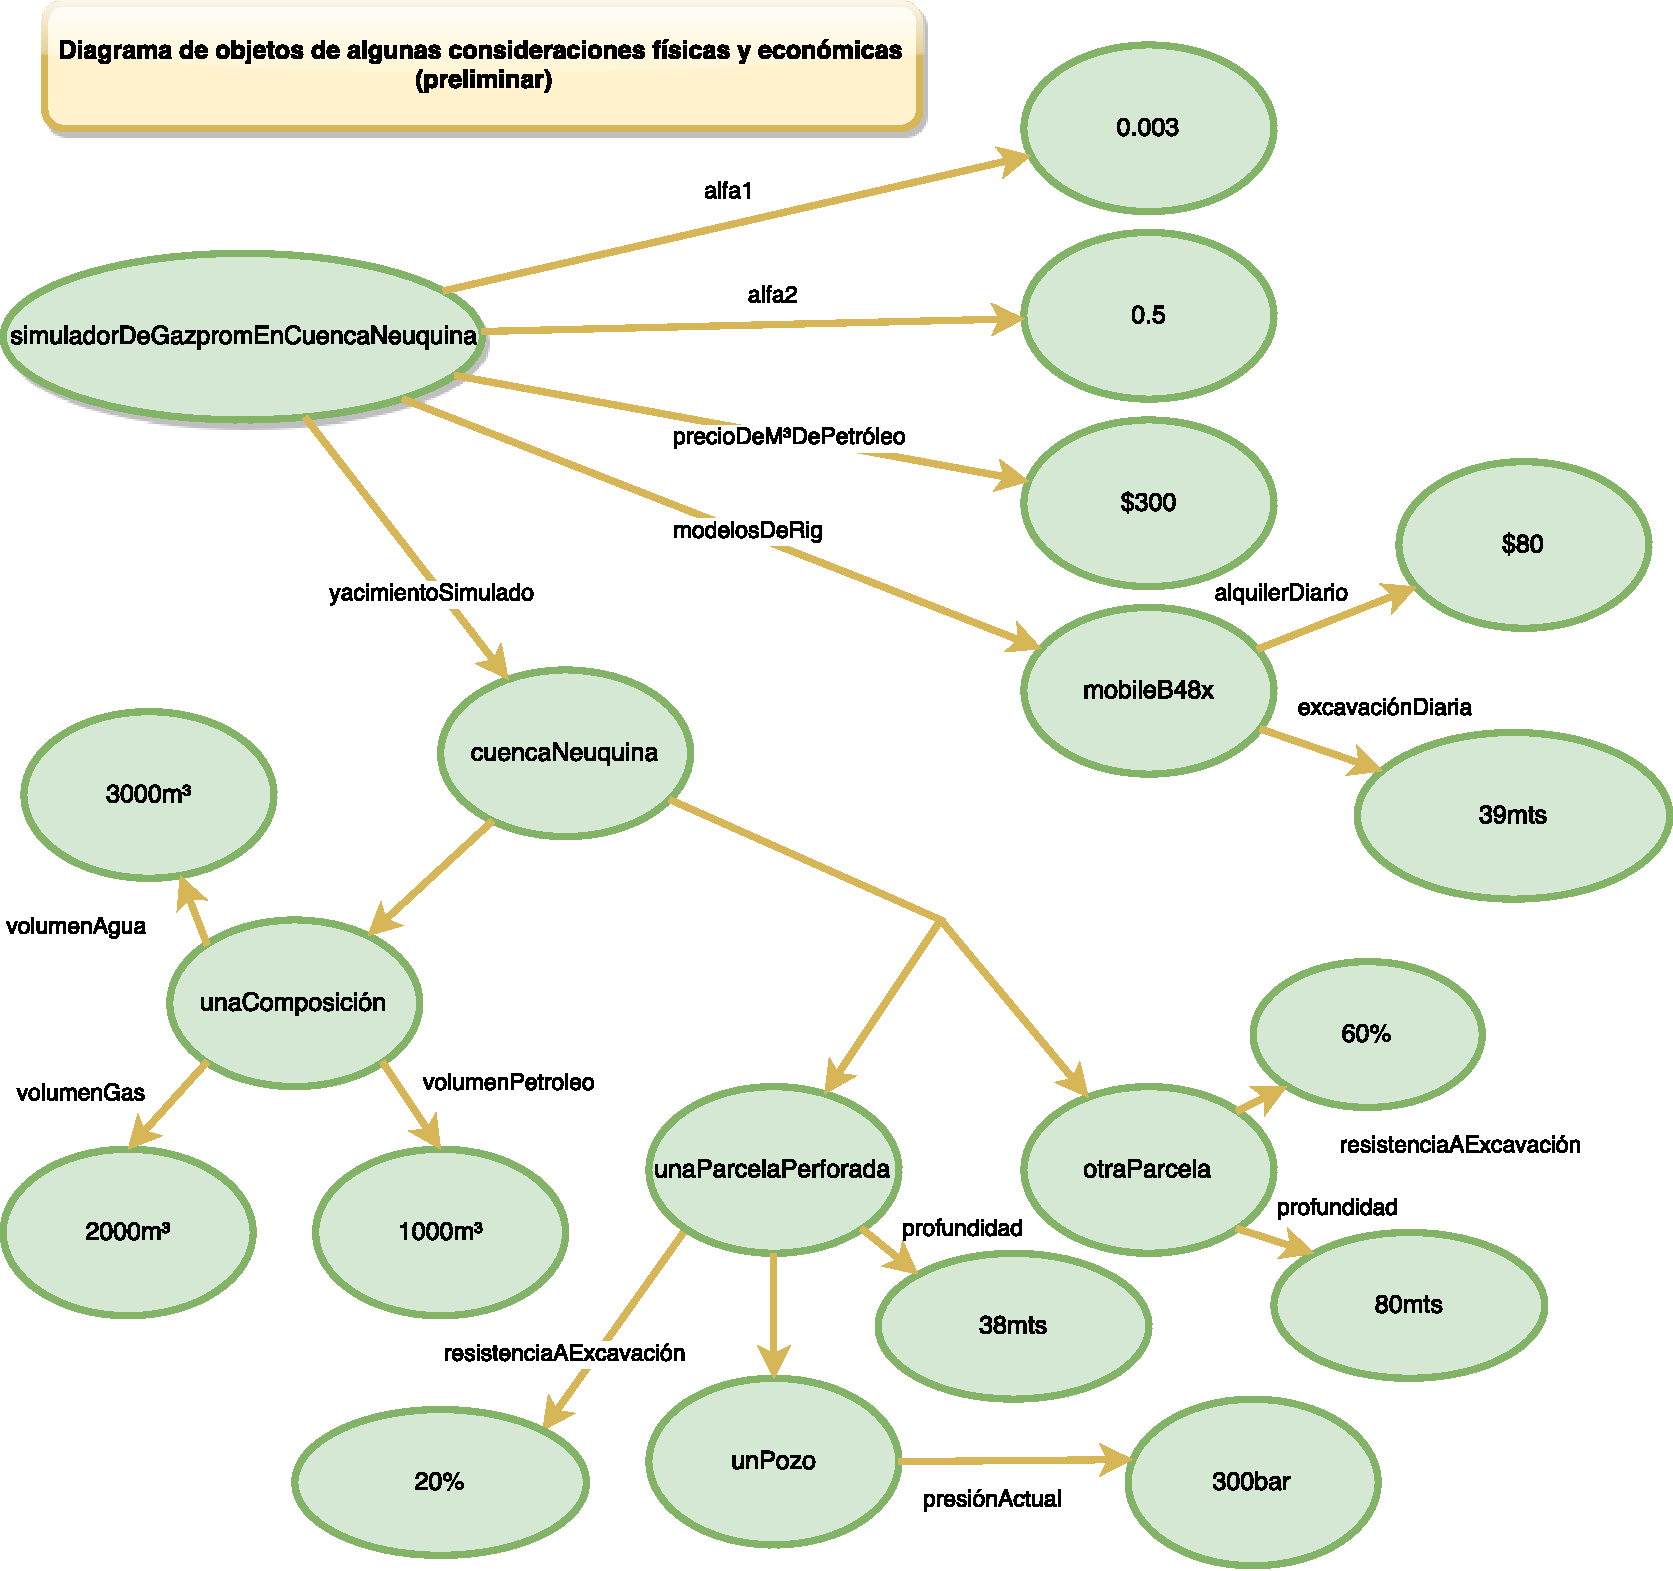
\includegraphics[width=\textwidth, height=\textheight, keepaspectratio]{objetos-modelado-fisico.pdf}
\end{figure}

Por un lado, planteamos que habría un objeto ``central'' que sería el mismo 
objeto que representa al simulador. Éste conocería otros como el objeto de un 
yacimiento, parámetros de configuración, los RIGS que tiene alquilados, plantas 
disponibles, entre otras cosas. Lo que se muestra en el diagrama es una visión 
parcial de la idea que teníamos en ese momento. 

Surgen otras nociones fundamentales, como por ejemplo que un yacimiento debería 
conocer otro objeto que representa la composición del mismo, o que las parcelas 
conocen a sus respectivos pozos en el caso de tener uno. Tratamos de mantener 
lo más posible un isomorfismo con la realidad en esta primera iteración. 

A esta altura sin embargo, y solo con este diagrama, no queda claro cómo es que 
se realizaría la ejecución propiamente dicha de la simulación. Tampoco por qué 
o cómo es que son seleccionadas las parcelas o RIGS para desempeñar tareas. \\

De lo especificado que debe realizar el simulador, se nos dice que es el equipo 
de ingeniería el responsable de tomar estas decisiones, y que lo hará mediante 
la elección de estrategias parametrizables para determinar diferentes criterios. 
Por ejemplo, debe poder elegirse el criterio que determina cuándo se deja de 
explotar un yacimiento, y este podría ser, por ejemplo, luego de una cantidad de 
tiempo fijo, o cuando la composición del yacimiento ya no es rentable. 

Nos surge entonces naturalmente la idea de representar estos \textbf{criterios} 
como objetos en sí mismo en nuestro diseño. A su vez, vemos que vamos a querer 
un diseño flexible respecto a cómo pueden ser estos criterios, porque para un 
criterio podríamos querer tener \textbf{muchas diferentes estrategias} (y además 
no conocemos todas con antelación). \\

Lo que decidimos entonces fue representar a cada tipo de criterio con una clase 
correspondiente, así tendremos la clase de los criterios de corte, la clase de 
los criterios de alquiler de RIGS, y así siguiendo. Además, queremos que quién 
utilice estos criterios (por ahora, el objeto del simulador) pueda abstraerse de 
si la estrategia que está utilizando es una u otra. Lo que vamos a hacer es 
mantener las clases de los criterios como abstractas, implementando una interfaz 
mínima que debe ofrecer ese criterio, y las distintas estrategias serán 
subclases de la misma. Veamos un ejemplo. 

\subsubsection{Diagrama de clases preliminar, criterios de corte}

\begin{figure}[H]
\centering
\caption{Fragmento diagrama de clases preliminar, para criterios de corte}
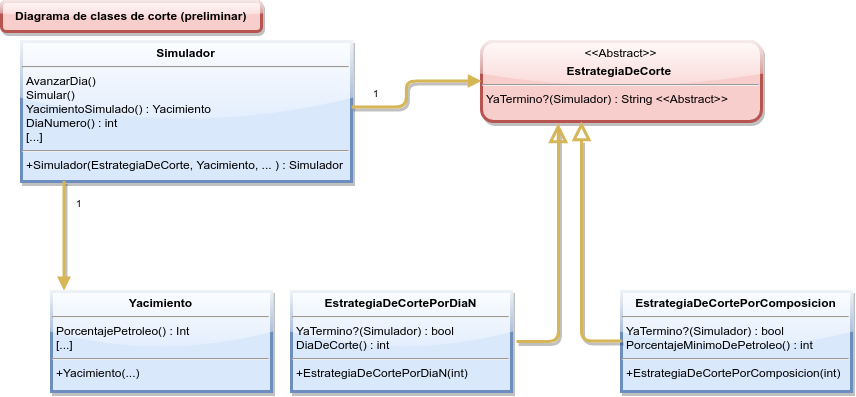
\includegraphics[width=0.95\textwidth, keepaspectratio]{clases-preliminar}
\end{figure}

Aquí puede verse la idea de la que hablábamos recién. En el ejemplo, la idea
es que todas las estrategias de corte sean polimórficas y puedan responder al 
mensaje \texttt{YaTermino?}, el cual le indicará al simulador si debe cortar 
con la simulación o no. Sin embargo éste no necesita saber con qué estrategia 
de corte está tratando. Esto se condice naturalmente con el patrón de diseño 
\textit{strategy} visto en la materia. \\

Mostramos a continuación un par de diagramas de secuencia siguiendo el ejemplo 
de las estrategias de corte, desarrollando cómo podría funcionar cada una. 

\subsubsection{Diagrama de secuencia de las estrategias de corte}

\begin{figure}[H]
\caption{Criterio de corte por cantidad de días, diseño preliminar}
\centering
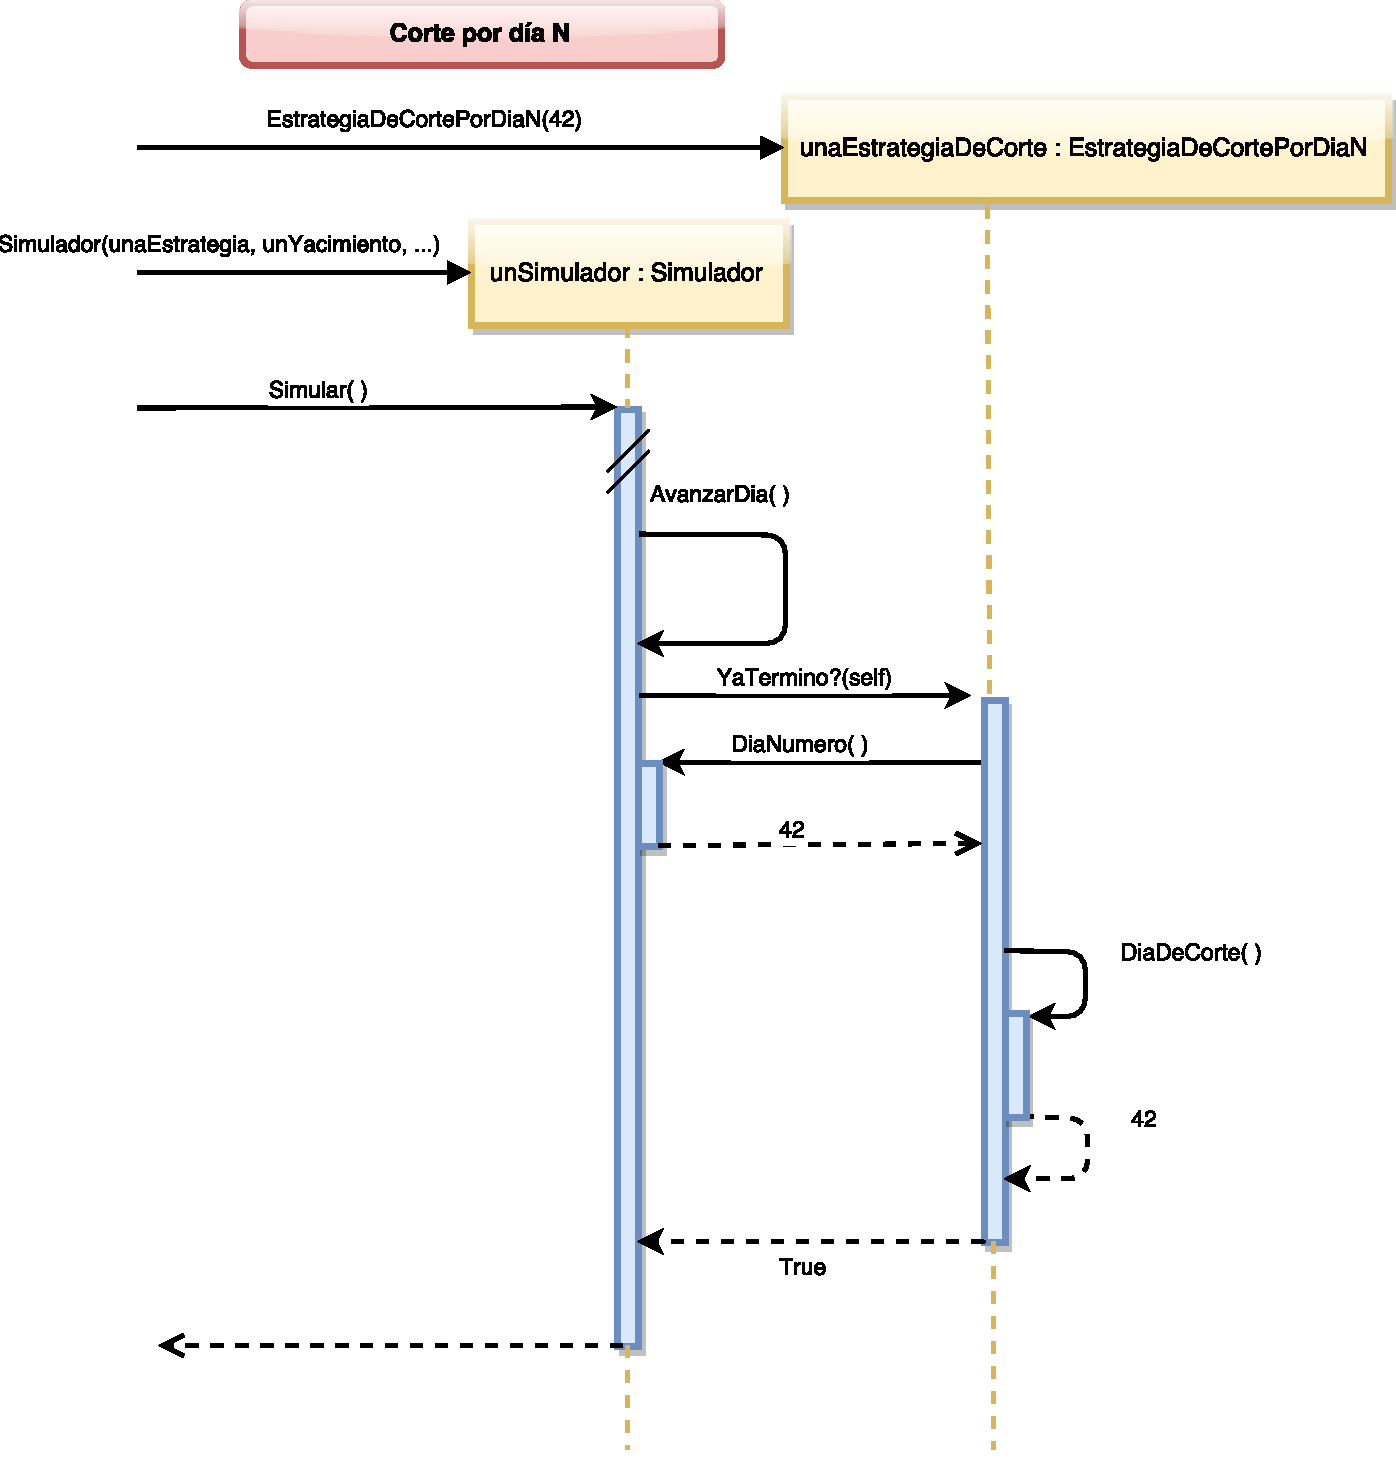
\includegraphics[width=\textwidth, height=\textheight, keepaspectratio]{secuencia-corte-dia.pdf}
\end{figure}

La secuencia comienza con el mensaje \texttt{Simular} del simulador. Éste 
internamente deberá ser responsable de avanzar un día en la simulación, con 
todo lo que eso conlleva, como la extracción de producto como la construcción 
de plantas o tanques. Entre esas, también necesita saber si debe terminar con la 
simulación, para esto le pregunta a su criterio de corte, que en este caso es 
fijo por cantidad de días, mediante el mensaje \texttt{YaTermino?}. El criterio 
de corte a su vez (como pasará con otros criterios) necesita poder conocer 
ciertas cosas del estado actual de la simulación, es por esto que dentro del 
mensaje \texttt{YaTermino?} el simulador en envía a sí mismo como colaborador. 
De esta manera luego el criterio de corte puede preguntarle el simulador 
cuál es el día actual de simulación. Con ese resultado, el criterio hace la 
comparación con su parámetro y devuelve su respuesta binaria. 

\begin{figure}[H]
\caption{Criterio de corte por composición del yacimiento, diseño preliminar}
\centering
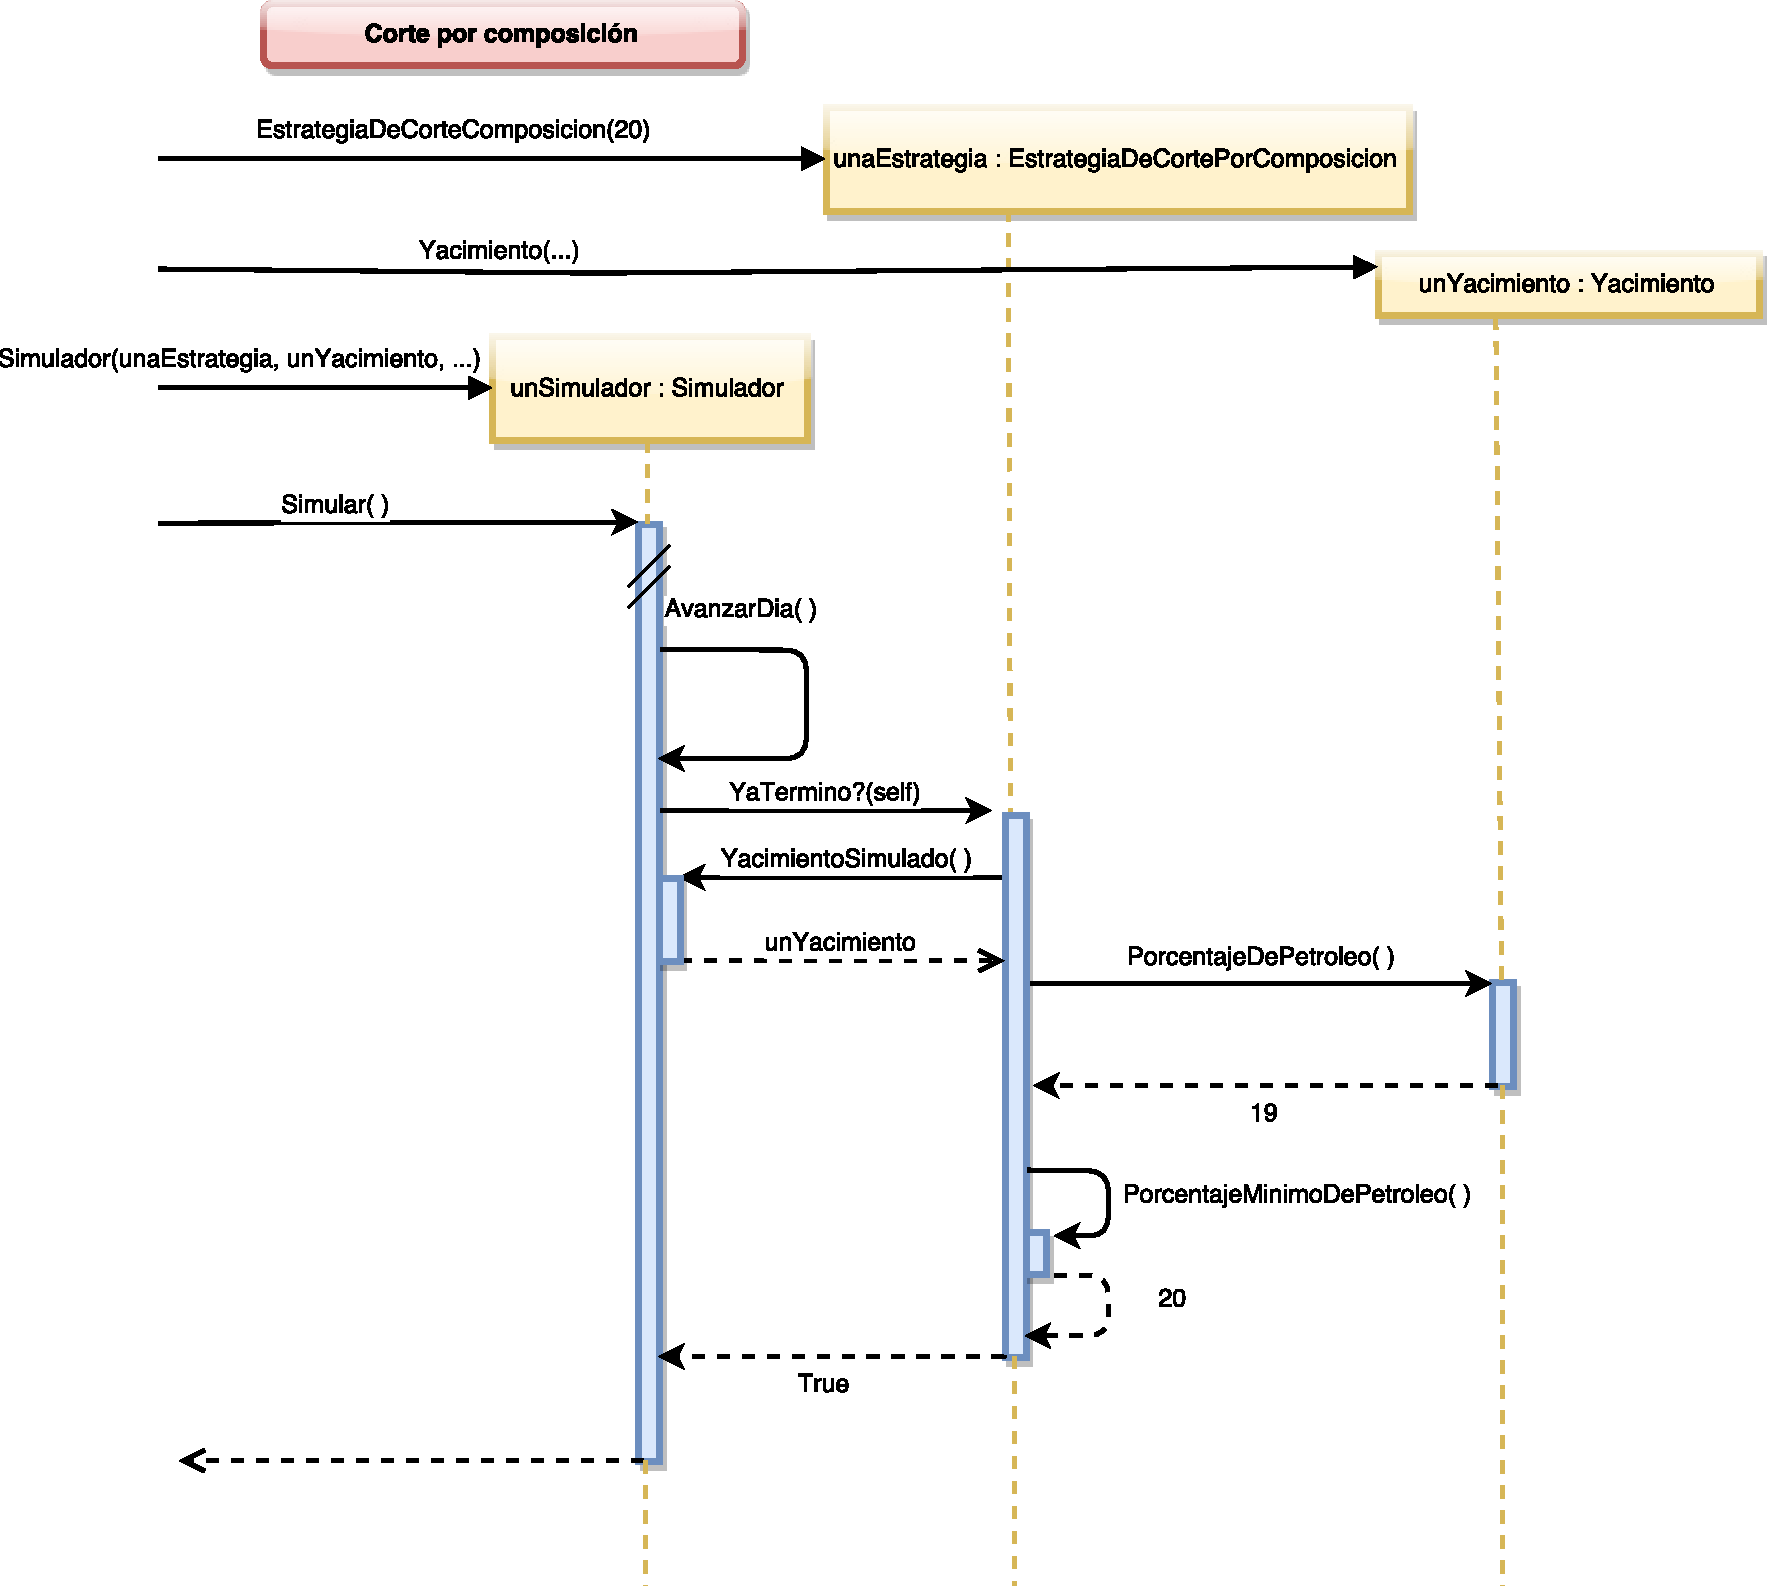
\includegraphics[width=\textwidth, height=\textheight, keepaspectratio]{secuencia-corte-composicion.pdf}
\end{figure}

Este otro diagrama se desarrolla de manera similar. La diferencia surge cuando 
el simulador envía el mensaje \texttt{YaTermino?} a su criterio de corte. 
Nuevamente, el simulador se envía a si mismo como colaborador del mensaje. En 
este caso, el criterio le pide al simulador por su yacimiento, mediante otro 
mensaje. Luego con el yacimiento obtiene la concentración de petróleo que hay en 
el mismo, compara con el valor mínimo aceptable, y devuelve la respuesta binaria. \\

Podemos ver entonces que mediante el uso de este patrón podemos mantener 
polimorfismo entre las diferentes estrategias de un mismo criterio, a la vez 
desacoplando la responsabilidad del simulador de la toma de decisiones del 
equipo de ingeniería. Por esto, decidimos conservar esta idea en lo que siguió 
de nuestra solución, que además fue un eje central para la misma. 

%%%%%%%%%%%%%%%%%%%% FIN? %%%%%%%%%%%%%%%%


\newpage

\subsection{Diseños finales}

\subsubsection{Diagrama de clases definitivo}
Presentamos ahora el diagrama de clases completo y definitivo  de nuestra solución. 
Lo mostramos separado en 3 partes que juntos hacen al total del diagrama. \\

\begin{figure}[H]
\centering
\caption{Diagrama de clases: clases del yacimiento}
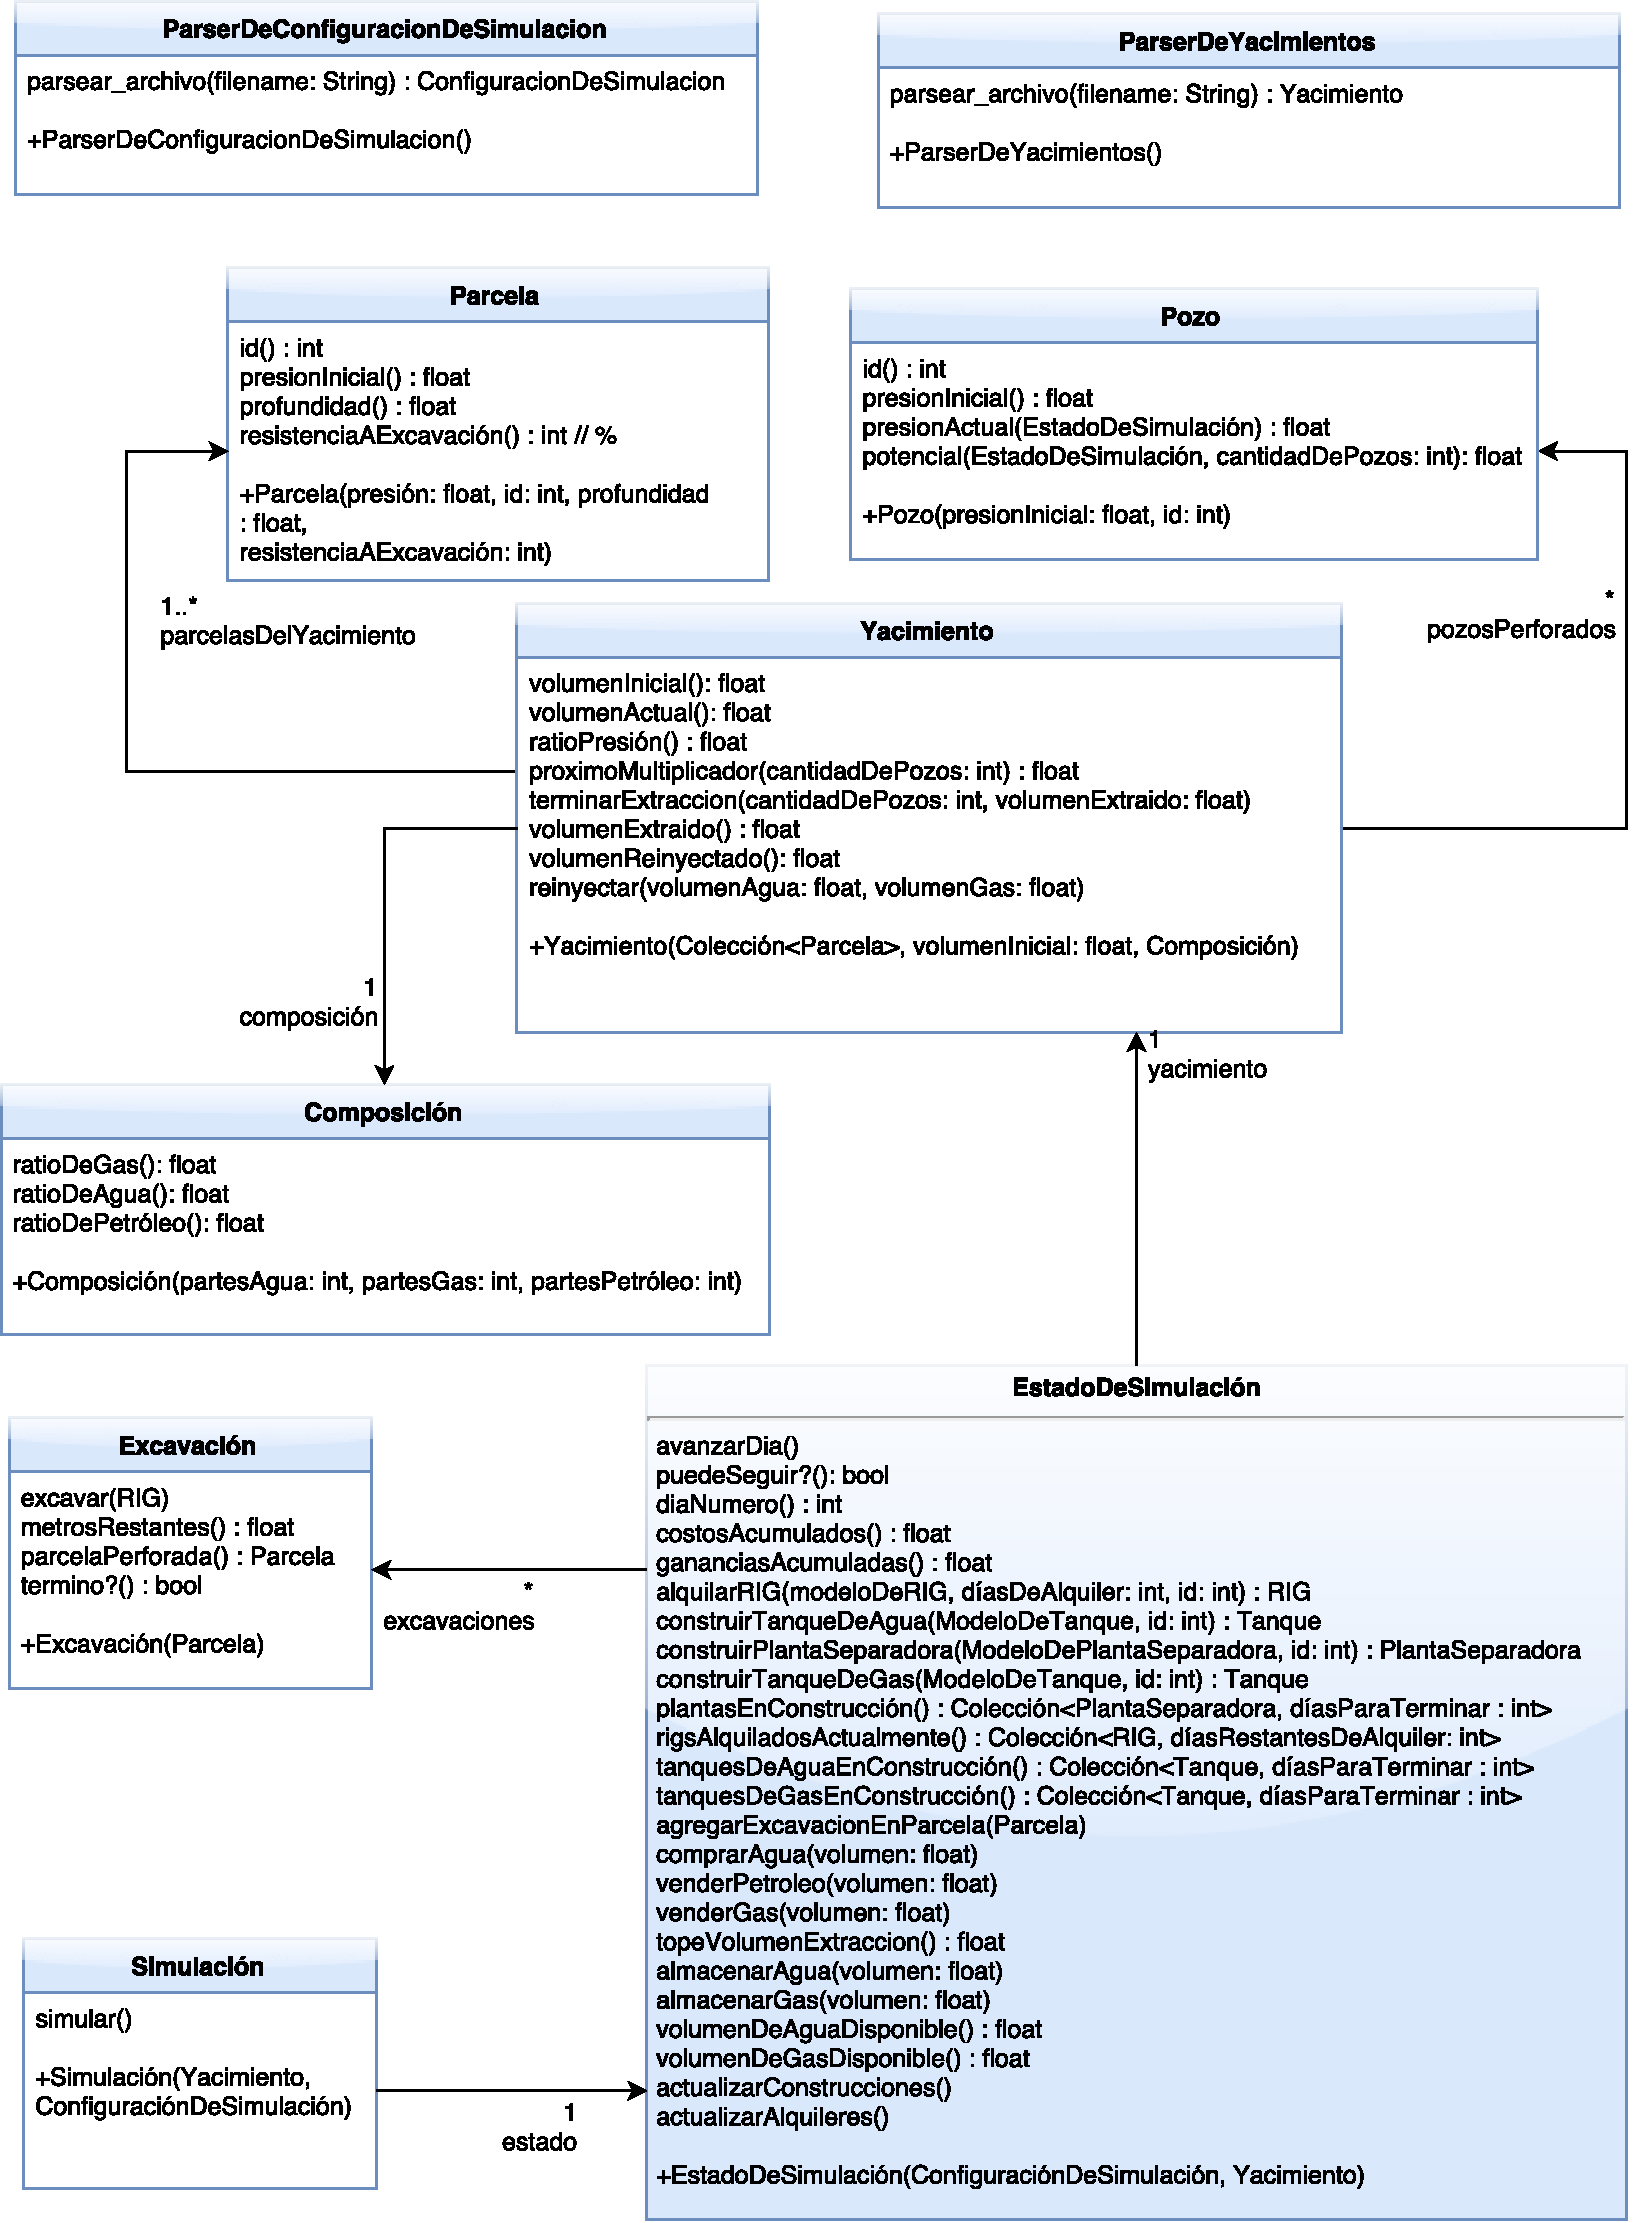
\includegraphics[width=0.95\textwidth, keepaspectratio]{clases-yacimiento}
\end{figure}

\newpage
\begin{figure}[H]
\centering
\caption{Diagrama de clases: clases de tanques, plantas separadoras y RIGS}
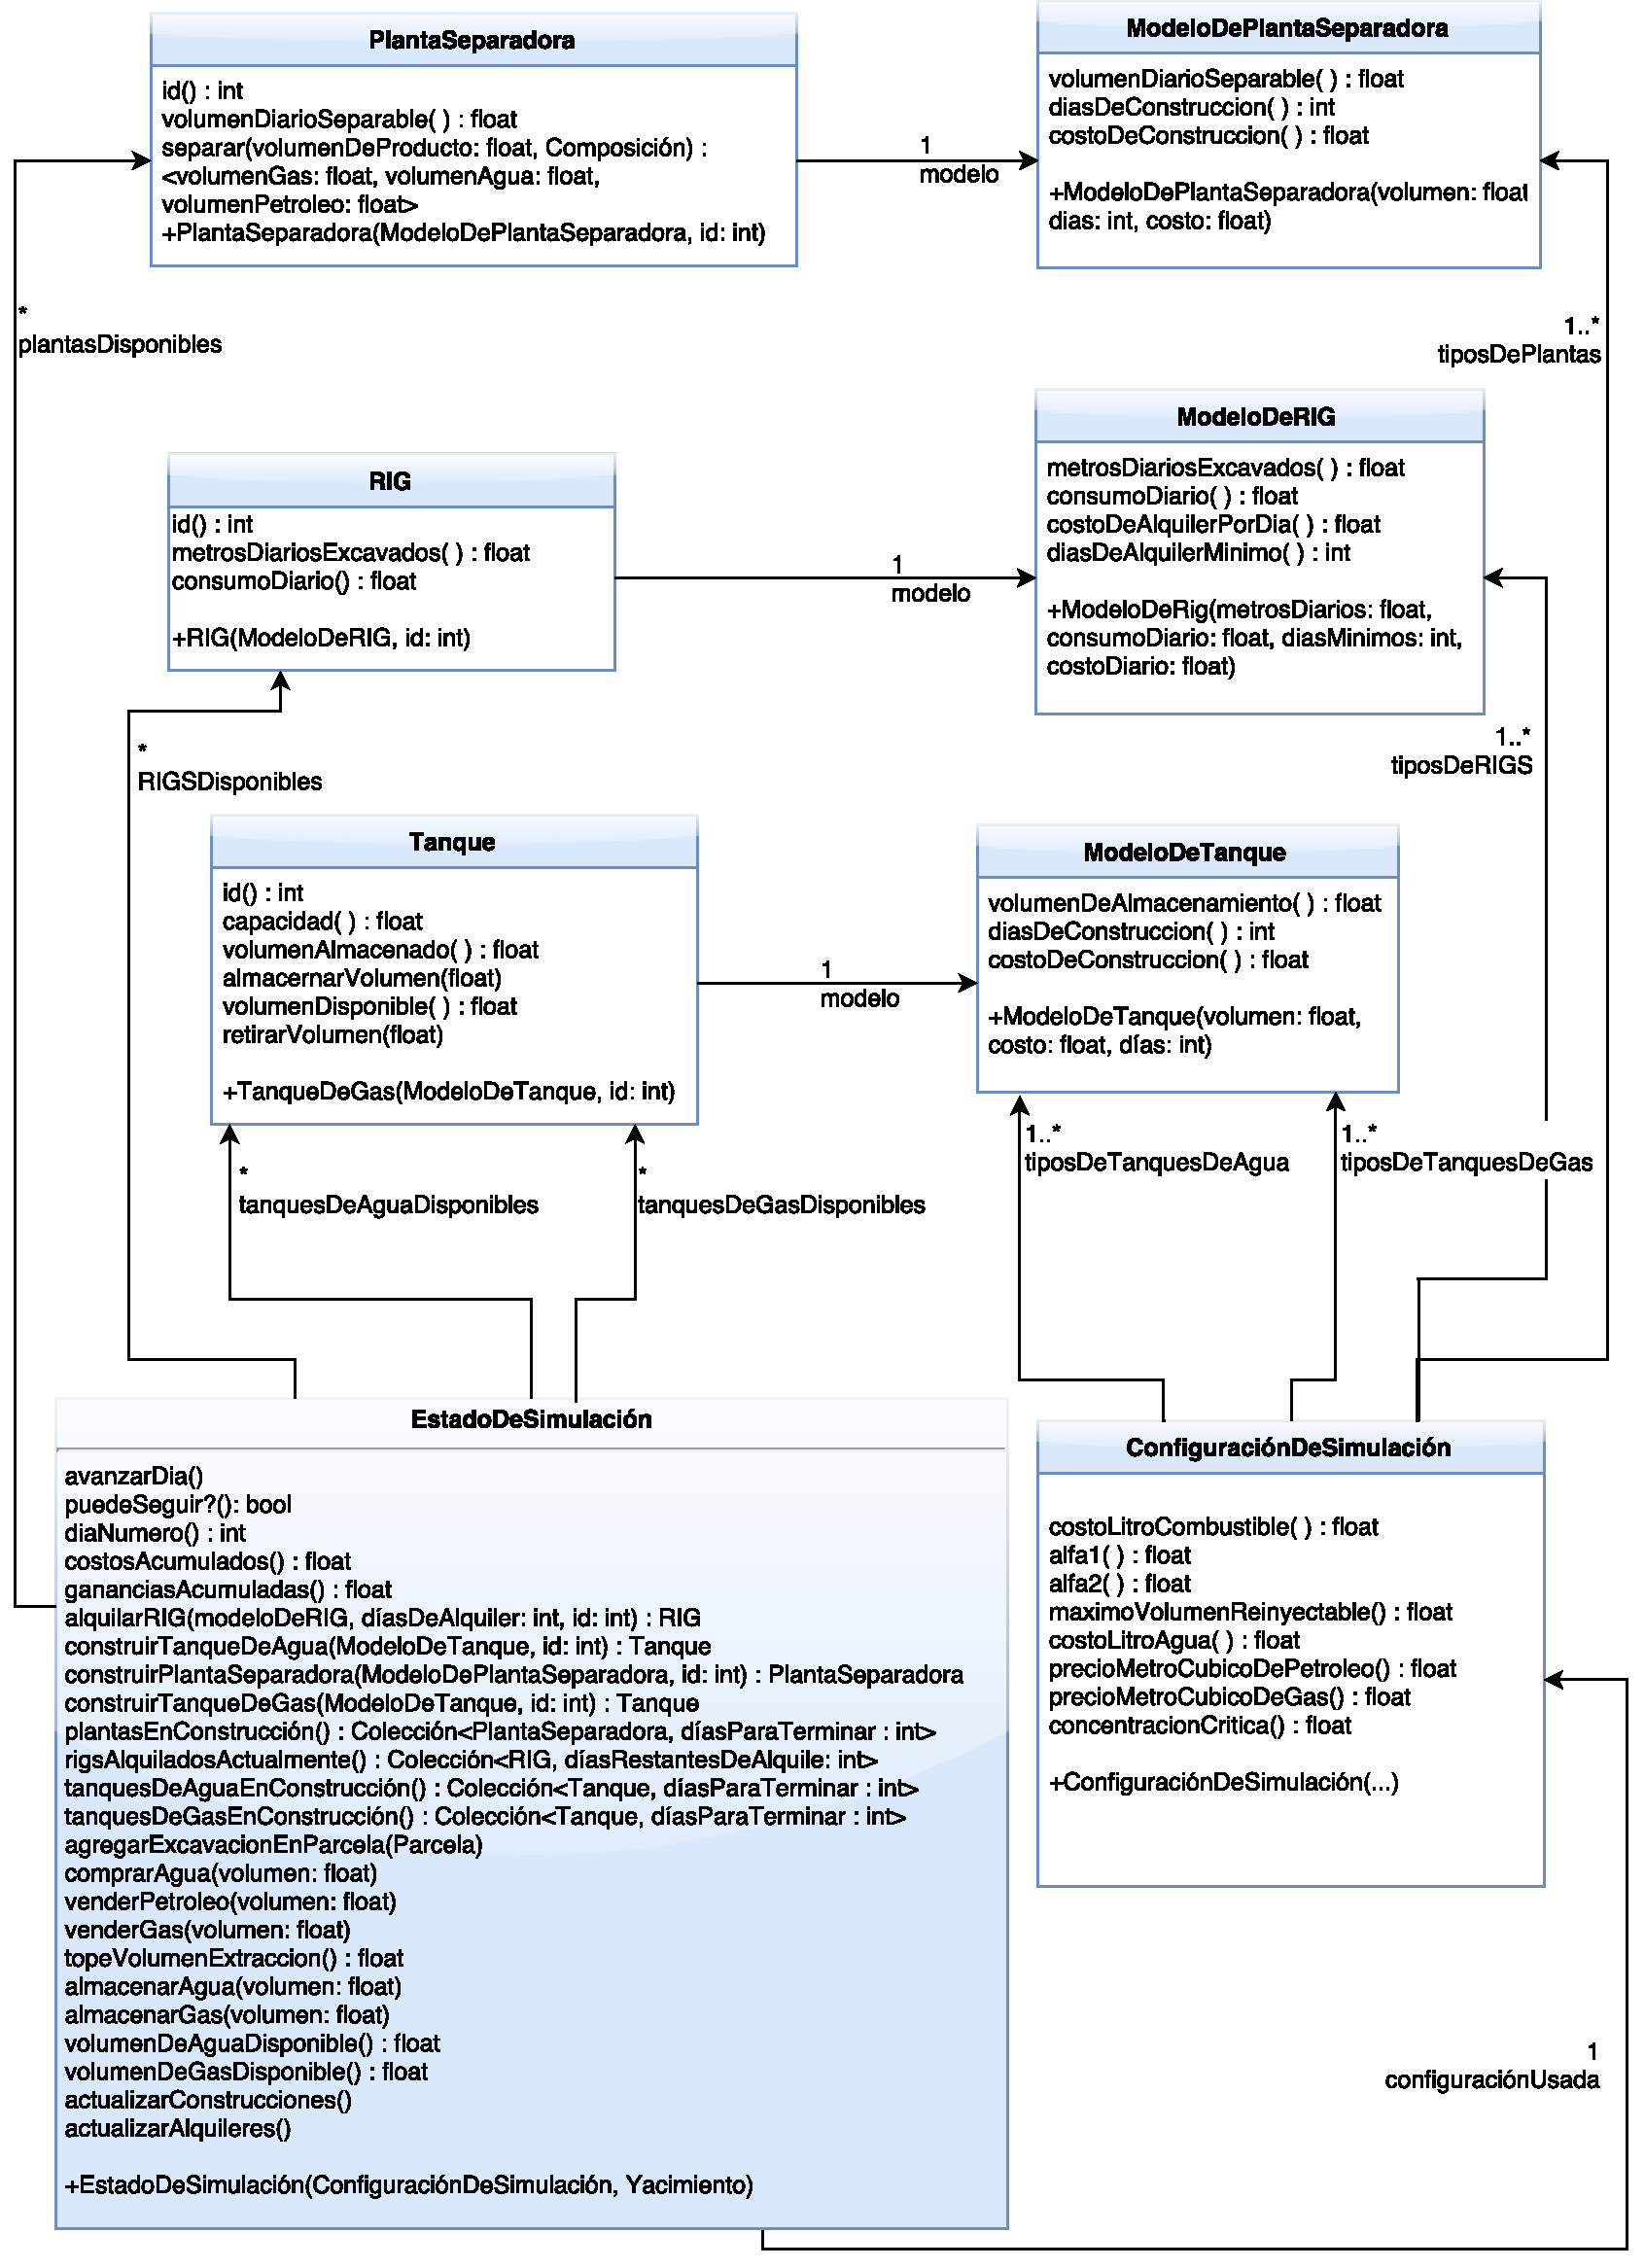
\includegraphics[width=0.95\textwidth, keepaspectratio]{clases-tanques-plantas}
\end{figure}

\newpage
\begin{figure}[H]
\centering
\caption{Diagrama de clases: clases de criterios del grupo de ingeniería}
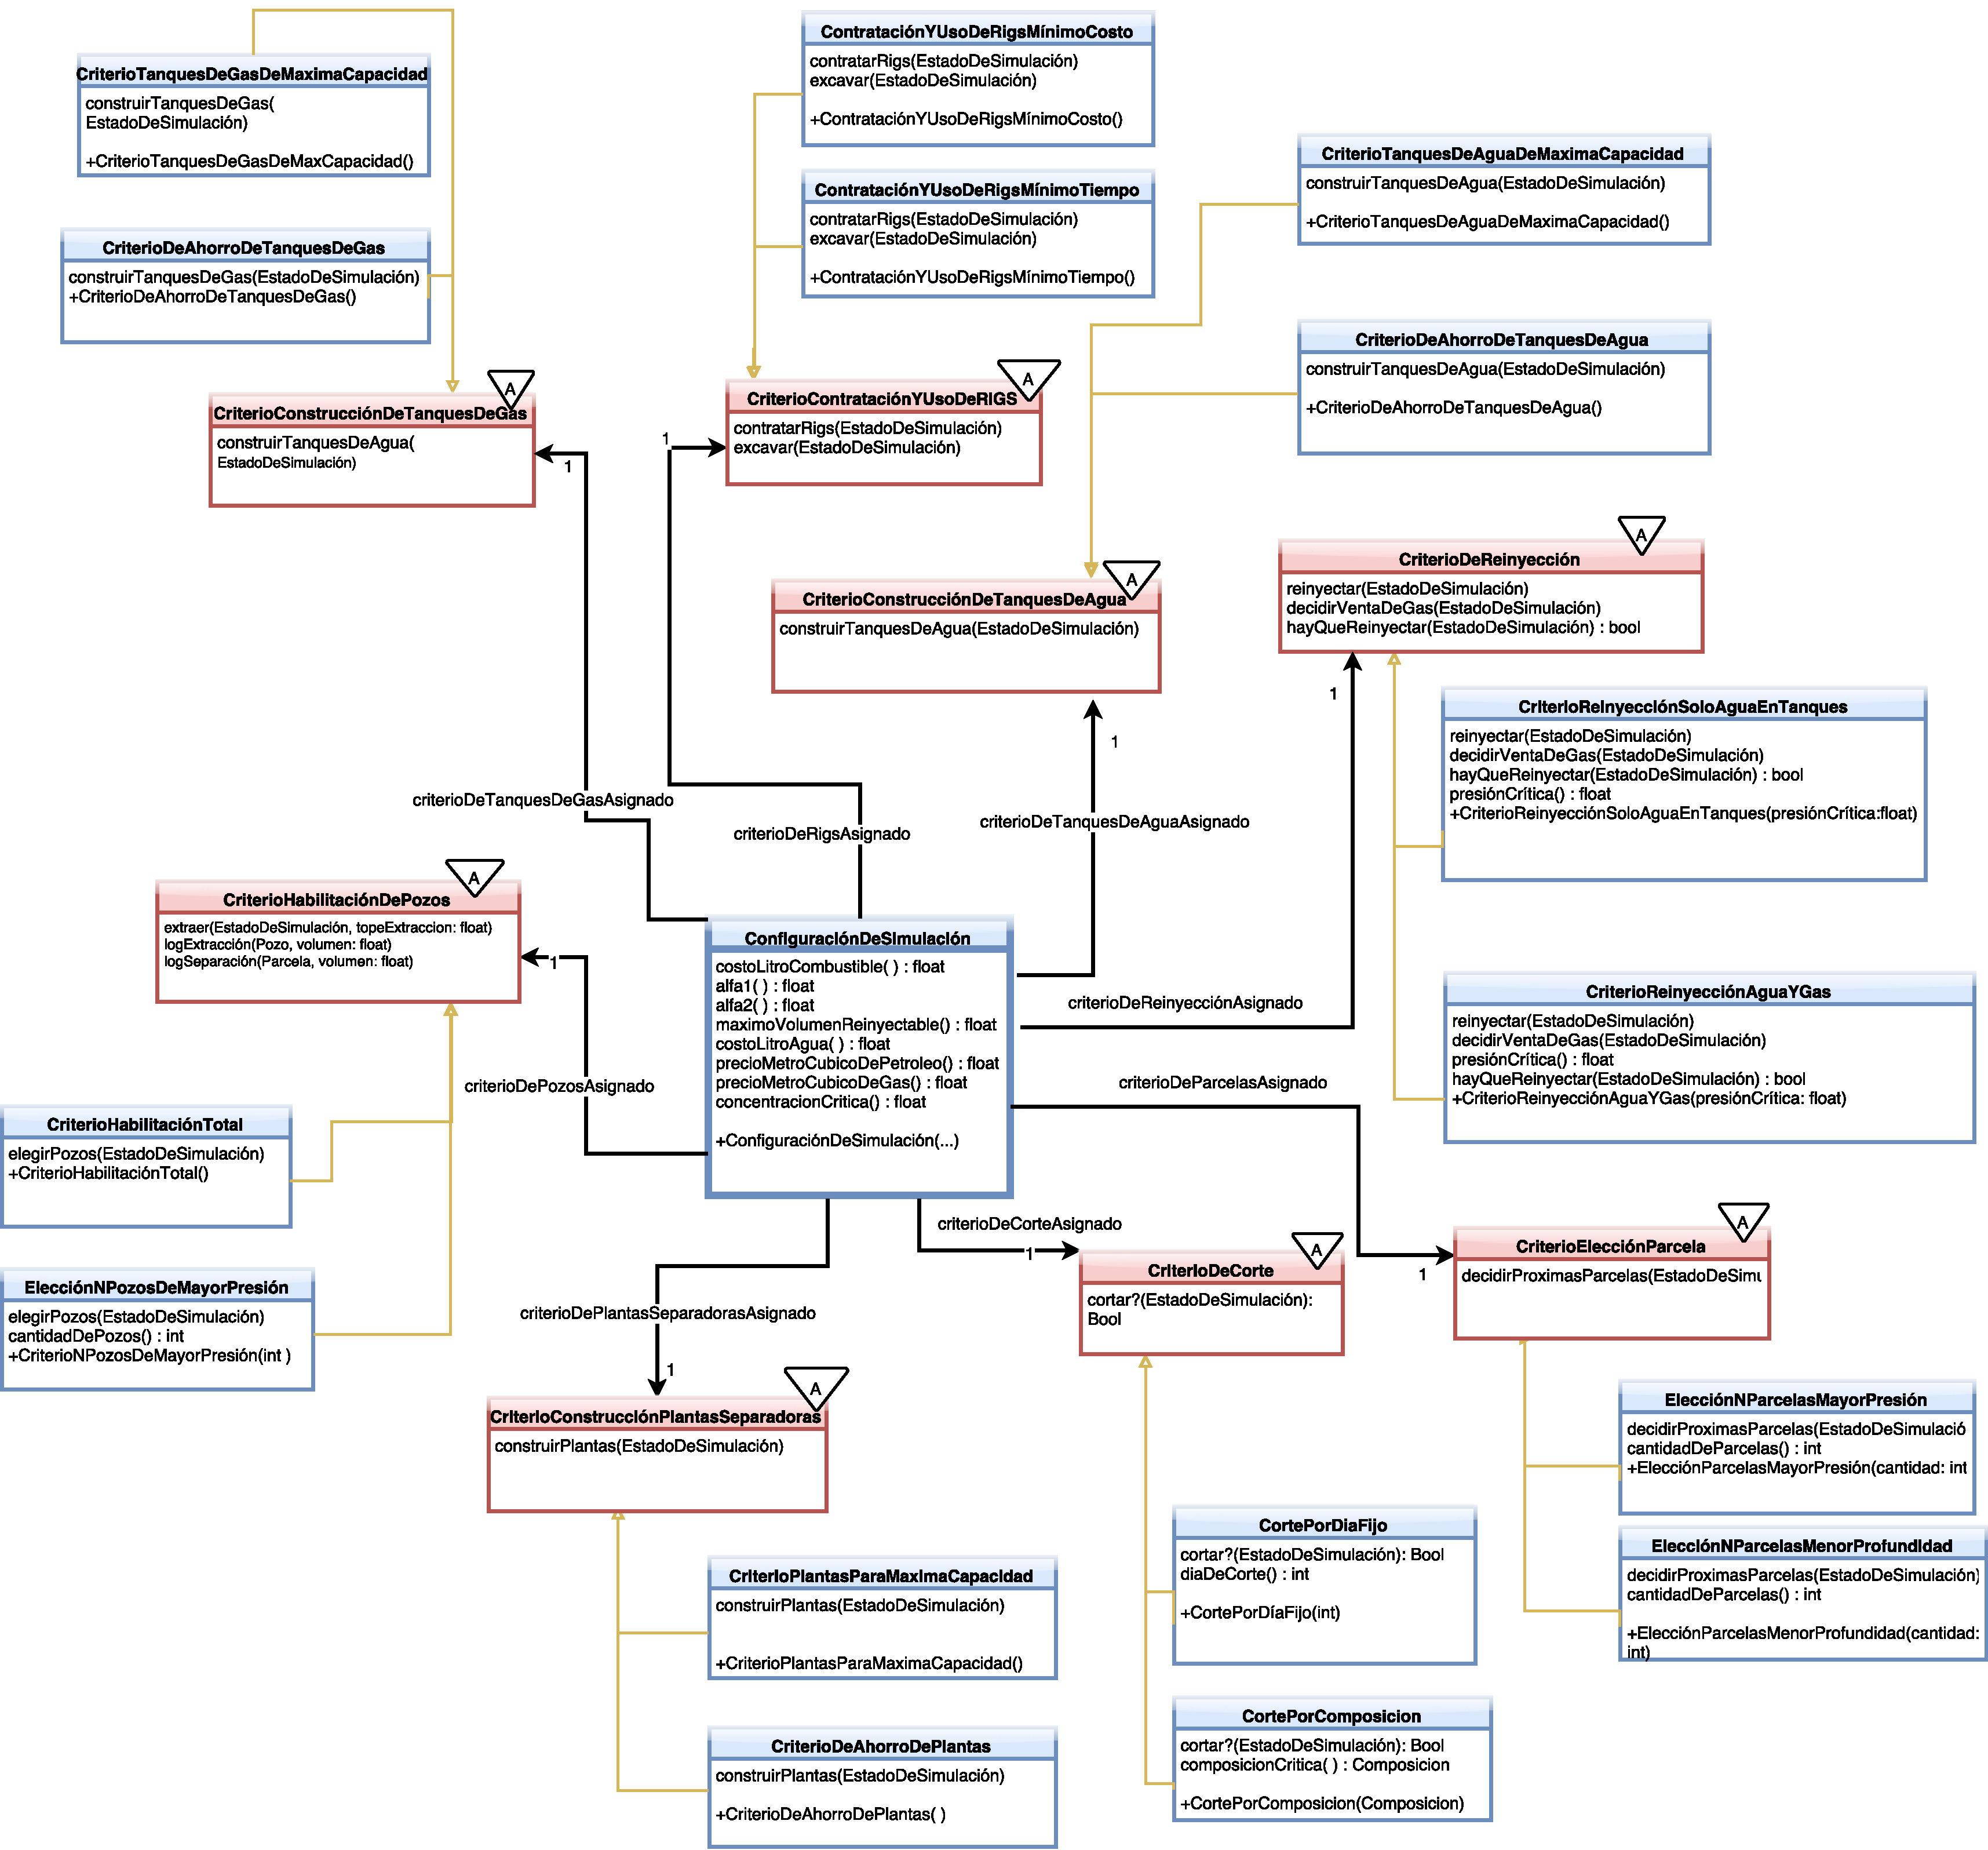
\includegraphics[width=1.10\textwidth, keepaspectratio]{clases-criterios}
\end{figure}

%%% desarrollo / explicacion 
Pueden apreciarse algunas diferencias entre el diagrama completo y las primeras 
ideas planteadas.

Por ejemplo, ahora el simulador no es el objeto central sino que simplemente es un cliente del EstadoDeSimulación, el cual sí ocupa dicho lugar central. 

Si bien se sigue con la idea de delegar decisiones a las clases de los criterios, el estado ahora no las conoce de primera mano, sino que estas son conocidas por una clase intermedia que representa la configuración de la simulación. 

Dicha clase actúa como un repositorio de los parámetros ingresados a la simulación. De esta manera el único eje de cambio del estado refiere a aspectos propios de la logística del día a día de la simulación (responder a alquileres, construcciones, ventas, etc), significando mayor cohesión.
\\

Los \emph{assets} (o recursos) de la simulación conocen un modelo y es a él a quien delegan los mensajes referentes a sus cualidades ``de fábrica''. Es responsabilidad de los criterios ir contando los números de id de sus construcciones y alquileres. Una alternativa a esto era consultarlos a la clase estado o que esta se encargara de ir contando cuando se le envían los mensajes de alquiler y construcción, pero nos pareció que no violaba la esencia de los criterios que se encargaran ellos mismos. 

Decidimos que modelar los tanques de agua y gas con una única clase, dado que es en su finalidad donde difieren. Responden a los mismos mensajes de la misma manera. Esto se asemeja a la realidad donde cisternas son utilizadas para almacenar diversos componentes.
\\

En un principio habíamos asociado cada pozo a su respectiva parcela, dado que en el mundo real \emph{los pozos están en las parcelas}, pero en el contexto de la simulación dicha asociación no aporta información y es irrelevante.
\\

Si bien podríamos haber hecho que la presión actual de un pozo fuera algo conocido por el mismo en todo momento y sea modificado día a día, decidimos que sea relativa al estado de la simulación. Esto se hace aprovechando el espíritu recursivo de las fórmulas de presión donde continuamente se multiplican valores sobre la presión inicial, dichos valores no dependen del pozo. 

Por lo tanto, el yacimiento conoce su \emph{ratioPresión} que representa las \emph{capas de multiplicación} de la fórmula recursiva, es decir, conserva el producto de todas las actualizaciones anteriores. Cuando se llama a \emph{presiónActual} de un pozo dado un estado, se multiplica la presión inicial por el ratio. Y día a día únicamente se actualiza el ratio multiplicándolo por $e^{-\beta_i}$ con $\beta_i$ definida como está en el enunciado.

Esto nos permite, en particular, que los pozos tengan esencia inmutable y que su presión esté ligada a un momento en particular de la simulación.
\\

La clase excavación representa parcelas en estado de perforación. Día  a día se actualizan los metros restantes hasta que llegan a 0, se anula la excavación y se agrega un nuevo pozo al yacimiento.
\\

Si bien no aporta información por ser una clase conocido por todos, existe tácitamente una clase logging que aporta el mensaje \emph{info} necesario para que el sistema pueda declarar, cuando haga falta, las acciones que se realizan. 
\\

En total, estos son todas las decisiones del equipo de ingeniería para las cuales 
desarrollamos \textbf{criterios} en forma de clases abstractas: 
\begin{itemize}
\item Elección de parcelas para excavación de pozos
\item Contratación de RIGS
\item Habilitación de pozos para extracción de producto
\item Construcción de plantas separadoras de producto
\item Construcción de tanques de agua
\item Construcción de tanques de gas
\item Reinyección 
\item Corte de explotación
\end{itemize}

Para cada uno de estos items, existe una clase correspondiente en nuestro modelo, 
cada una con un par de alternativas de estrategias. \\

Para los criterios que deciden construcciones, excavaciones o alquileres, decidimos implementar estrategias que decidan únicamente el primer día todo lo necesario para el resto de la explotación. Siendo criterios \emph{dummy} el resto de los días. \\

En la sección siguiente mostramos y explicamos algunos diagramas de secuencia 
de distintas partes del simulador, para entender mejor el funcionamiento interno 
del mismo y cómo nuestro diseño queda implementado finalmente. 

%%%%%%%%%%%%%%%%%%%%%%%%%%%%%%%%%%%%%%%%%%%%%%%%%
%%%%%%%%%%%%%%%%%%%%%%%%%%%%%%%%%%%%%%%%%%%%%%%%%
%%%%%%%%%%%%%%%%%%%%%%%%%%%%%%%%%%%%%%%%%%%%%%%%%

\newpage
\subsubsection{Diagramas de secuencia}
\textbf{Diagrama de avanzarDia}
\begin{figure}[H]
\centering
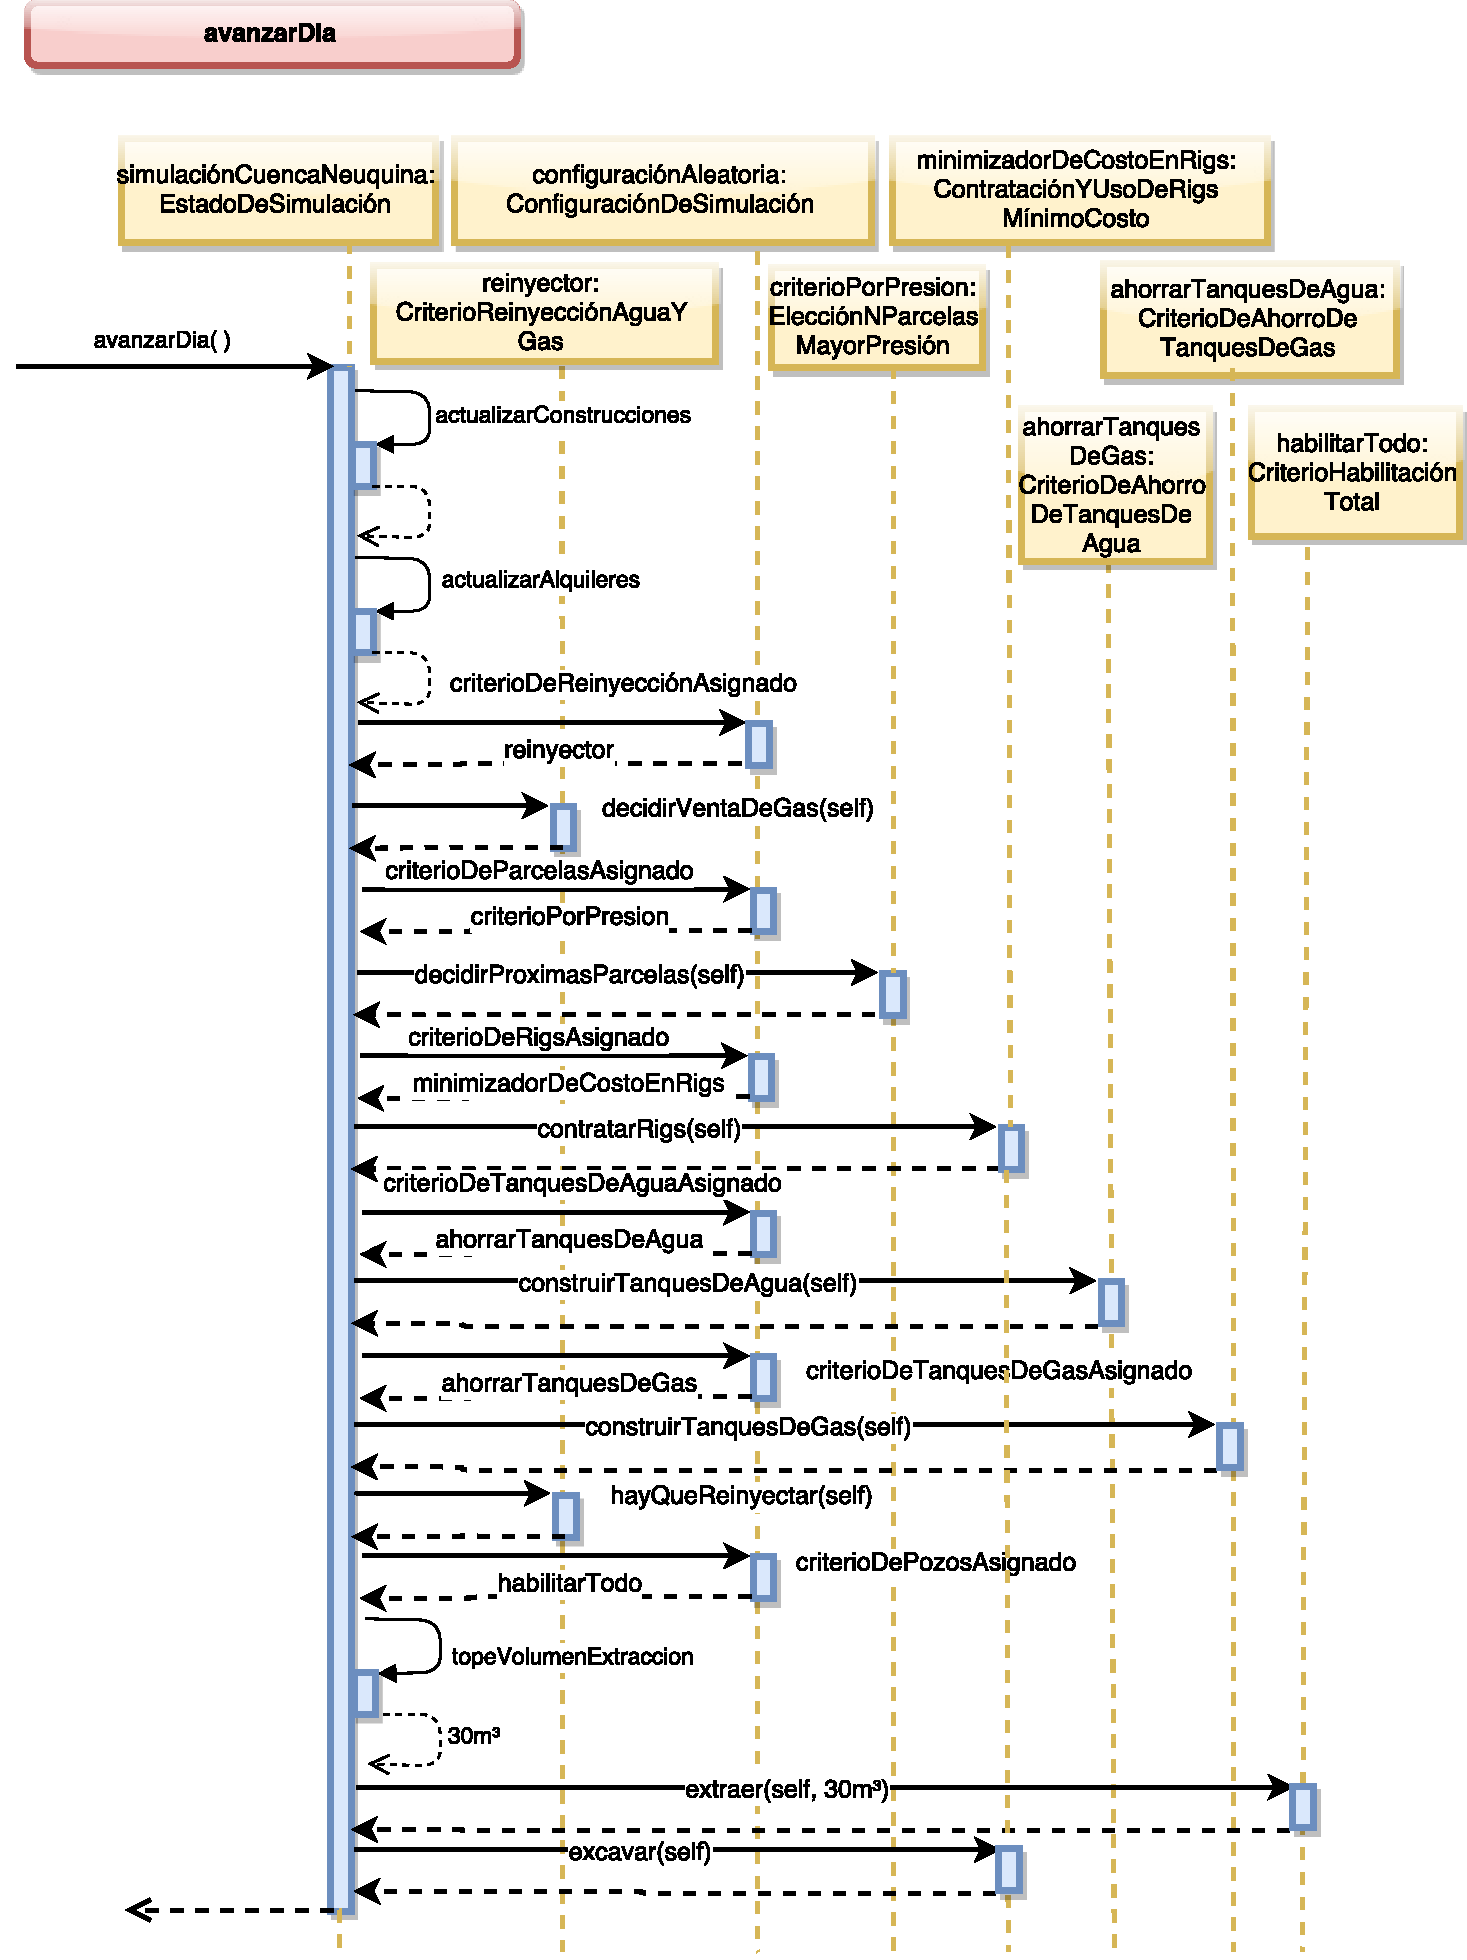
\includegraphics[width=1\textwidth, keepaspectratio]{avanzardia}
\end{figure}
La dinámica de la simulación está centrada en el mensaje \texttt{avanzarDia} del \texttt{EstadoDeSimulación}. Durante dicho mensaje, el estado se encarga de iniciar colaboraciones con todos los criterios para que se encarguen de hacer todos los cambios necesarios para desarrollar las funcionalidades del simulador (por ejemplo, 
empezar excavaciones, construcciones, habilitar pozos para extraer producto). 
\\

De esta manera, el estado se encarga únicamente de actualizar el día y los tiempos restantes de las construcciones y alquileres (y haciendo lo necesario en caso de que terminen). Los demás cambios en el sistema los comandan los criterios elegidos, en conocimiento del estado. Esto tiene sentido, dado que son las decisiones del día a día del equipo de ingeniería las que determinan el flujo y resultado de la simulación.
\\

\newpage
\textbf{Diagrama de secuencia de distintos tipos de criterios}

A continuación detallaremos con diagramas de secuencia algunas de las decisiones y colaboraciones que realizan los criterios definidos.
\\
%%%%%%%%%%%%%%%%%%%%%%%%%%%%%%%%%%%%%%%%%%%%%%%%%

\textbf{Diagrama de criterio de corte}
\begin{figure}[H]
\centering
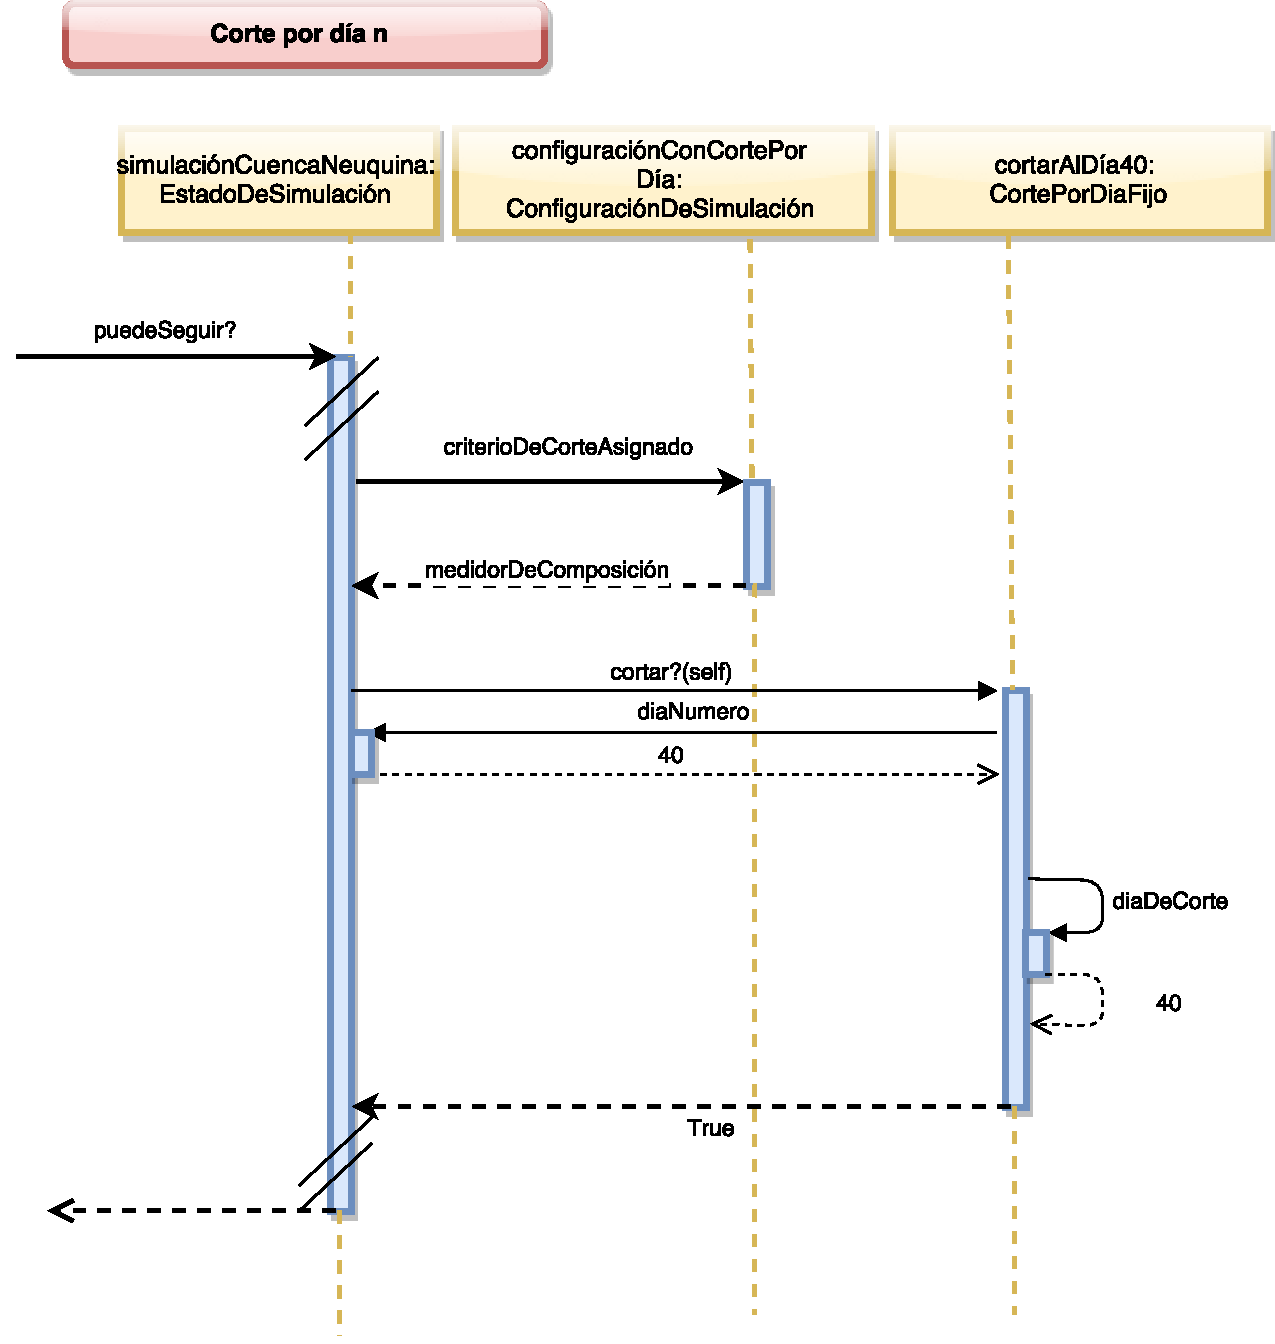
\includegraphics[width=1\textwidth, keepaspectratio]{corte}
\end{figure}

Durante la simulación, la clase \texttt{Simulación} se encarga constantemente 
de preguntarle al estado si debe continuar la simulación, mediante el mensaje 
\texttt{puedeSeguir?}. En caso de retornar \texttt{True}, la simulación 
le envía el mensaje \texttt{avanzarDía} al estado. 

Para el estado poder responder a esto, compara la proporción de petróleo en el 
yacimiento con el umbral mínimo permitido, y además utiliza su criterio de corte. 
Los criterios de corte solo están obligados a responder el 
mensaje \texttt{cortar?}. 

Este diagrama presenta un escenario en el cual el estado recibe el mensaje \texttt{puedeSeguir?}. En este caso, el criterio de corte por día fijo, en particular, 40. Por lo tanto el criterio decide que es necesario cortar. 

En el caso de un corte únicamente por composición, el criterio compararía a su vez también su propia composición crítica con la composición actual del yacimiento.

%%%%%%%%%%%%%%%%%%%%%%%%%%%%%%%%%%%%%%%%%%%%%%%%%

\newpage
\textbf{Diagrama de criterio de reinyección}
\begin{figure}[H]
\centering
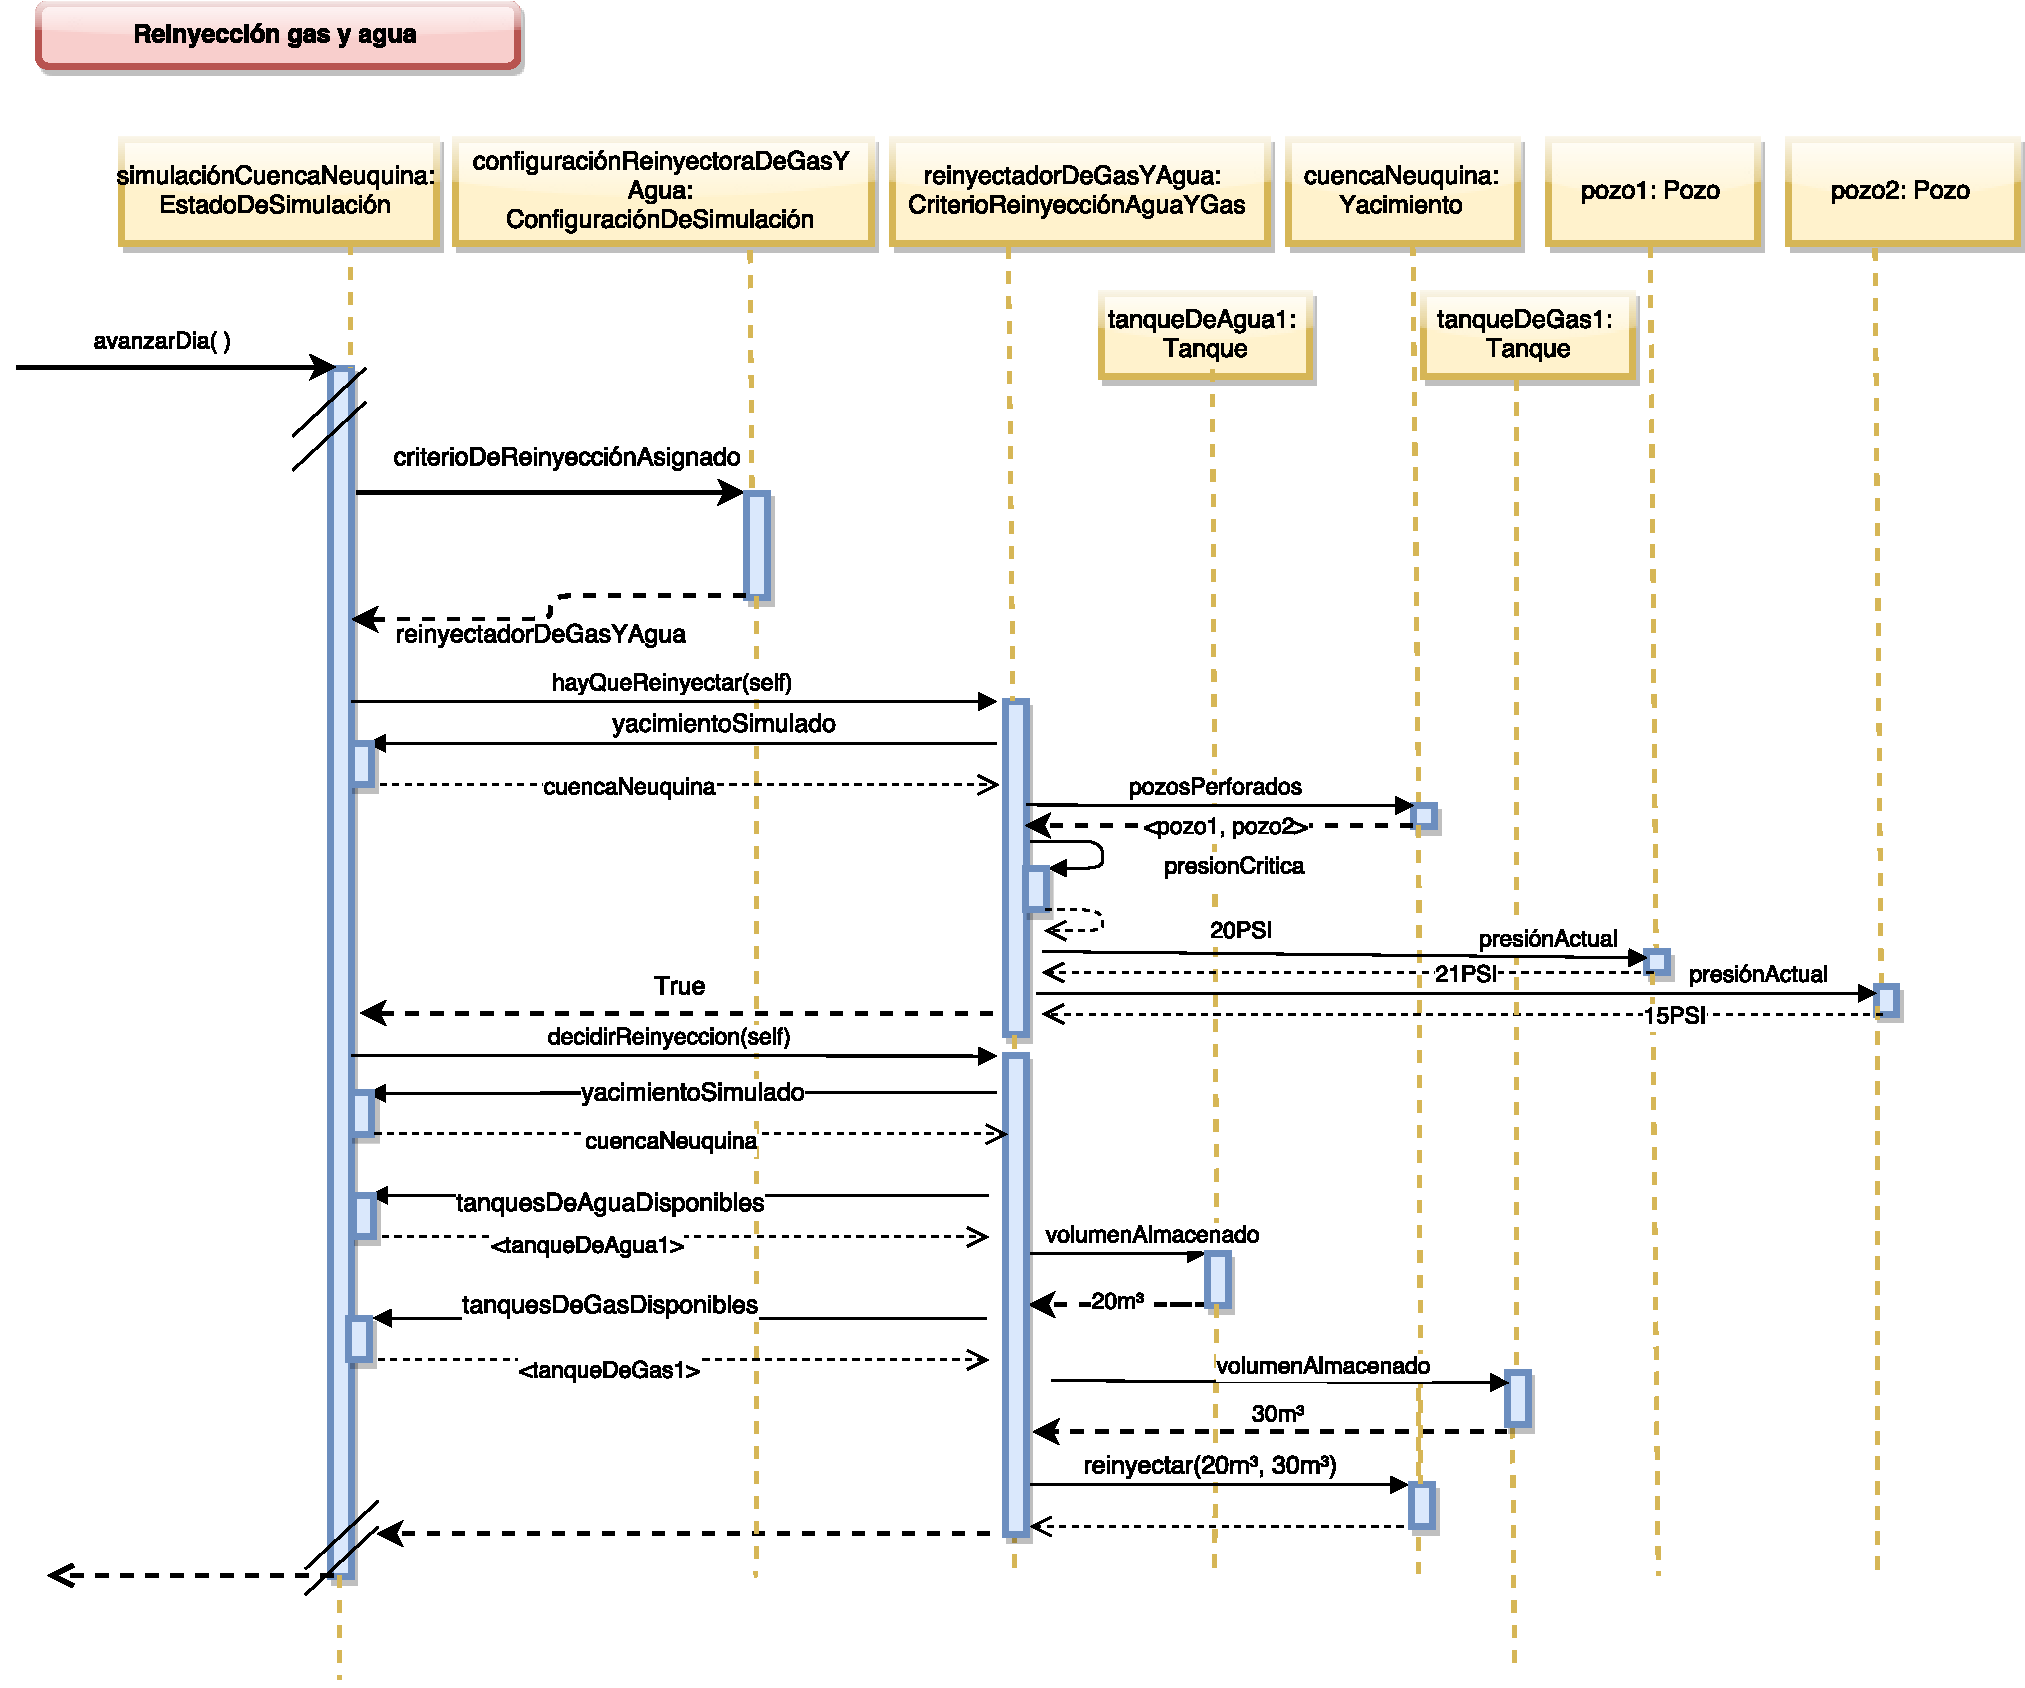
\includegraphics[width=1.15\textwidth, keepaspectratio]{reinyeccion}
\end{figure}

Dentro de \texttt{avanzarDía} del estado de simulación, se utiliza el criterio de 
reinyección seleccionado. Los criterios de reinyección deben saber responder a 3 
mensajes: \texttt{decidirVentaGas}, \texttt{hayQueReinyectar} y 
\texttt{reiyectar}. 


El escenario de la reinyección trata de una simulación configurada para reinyectar tanto gas como agua almacenada (nunca compra). Como el criterio reinyecta todo el agua y gas disponibles en tanques, al contar con un único tanque de cada tipo reinyecta su volumen almacenado. 
\\

El criterio decide reinyectar al recibir el mensaje \texttt{hayQueReinyectar} al notar que existe al menos un pozo con presión menor que la presión umbral seteada.
\\

Si bien al momento de reinyectar usa todo el gas, el criterio implementa el mensaje \texttt{venderGas} de modo que guarde la mitad para las reinyecciones. En el caso del criterio de reinyección de solo agua almacenada, el gas es vendido en su totalidad, y las colaboraciones para reinyectar son las mismas pero obviando la consulta a tanques de gas. 

%%%%%%%%%%%%%%%%%%%%%%%%%%%%%%%%%%%%%%%%%%%%%%%%%

\newpage
\textbf{Diagrama de criterio de construcción de plantas}
\begin{figure}[H]
\centering
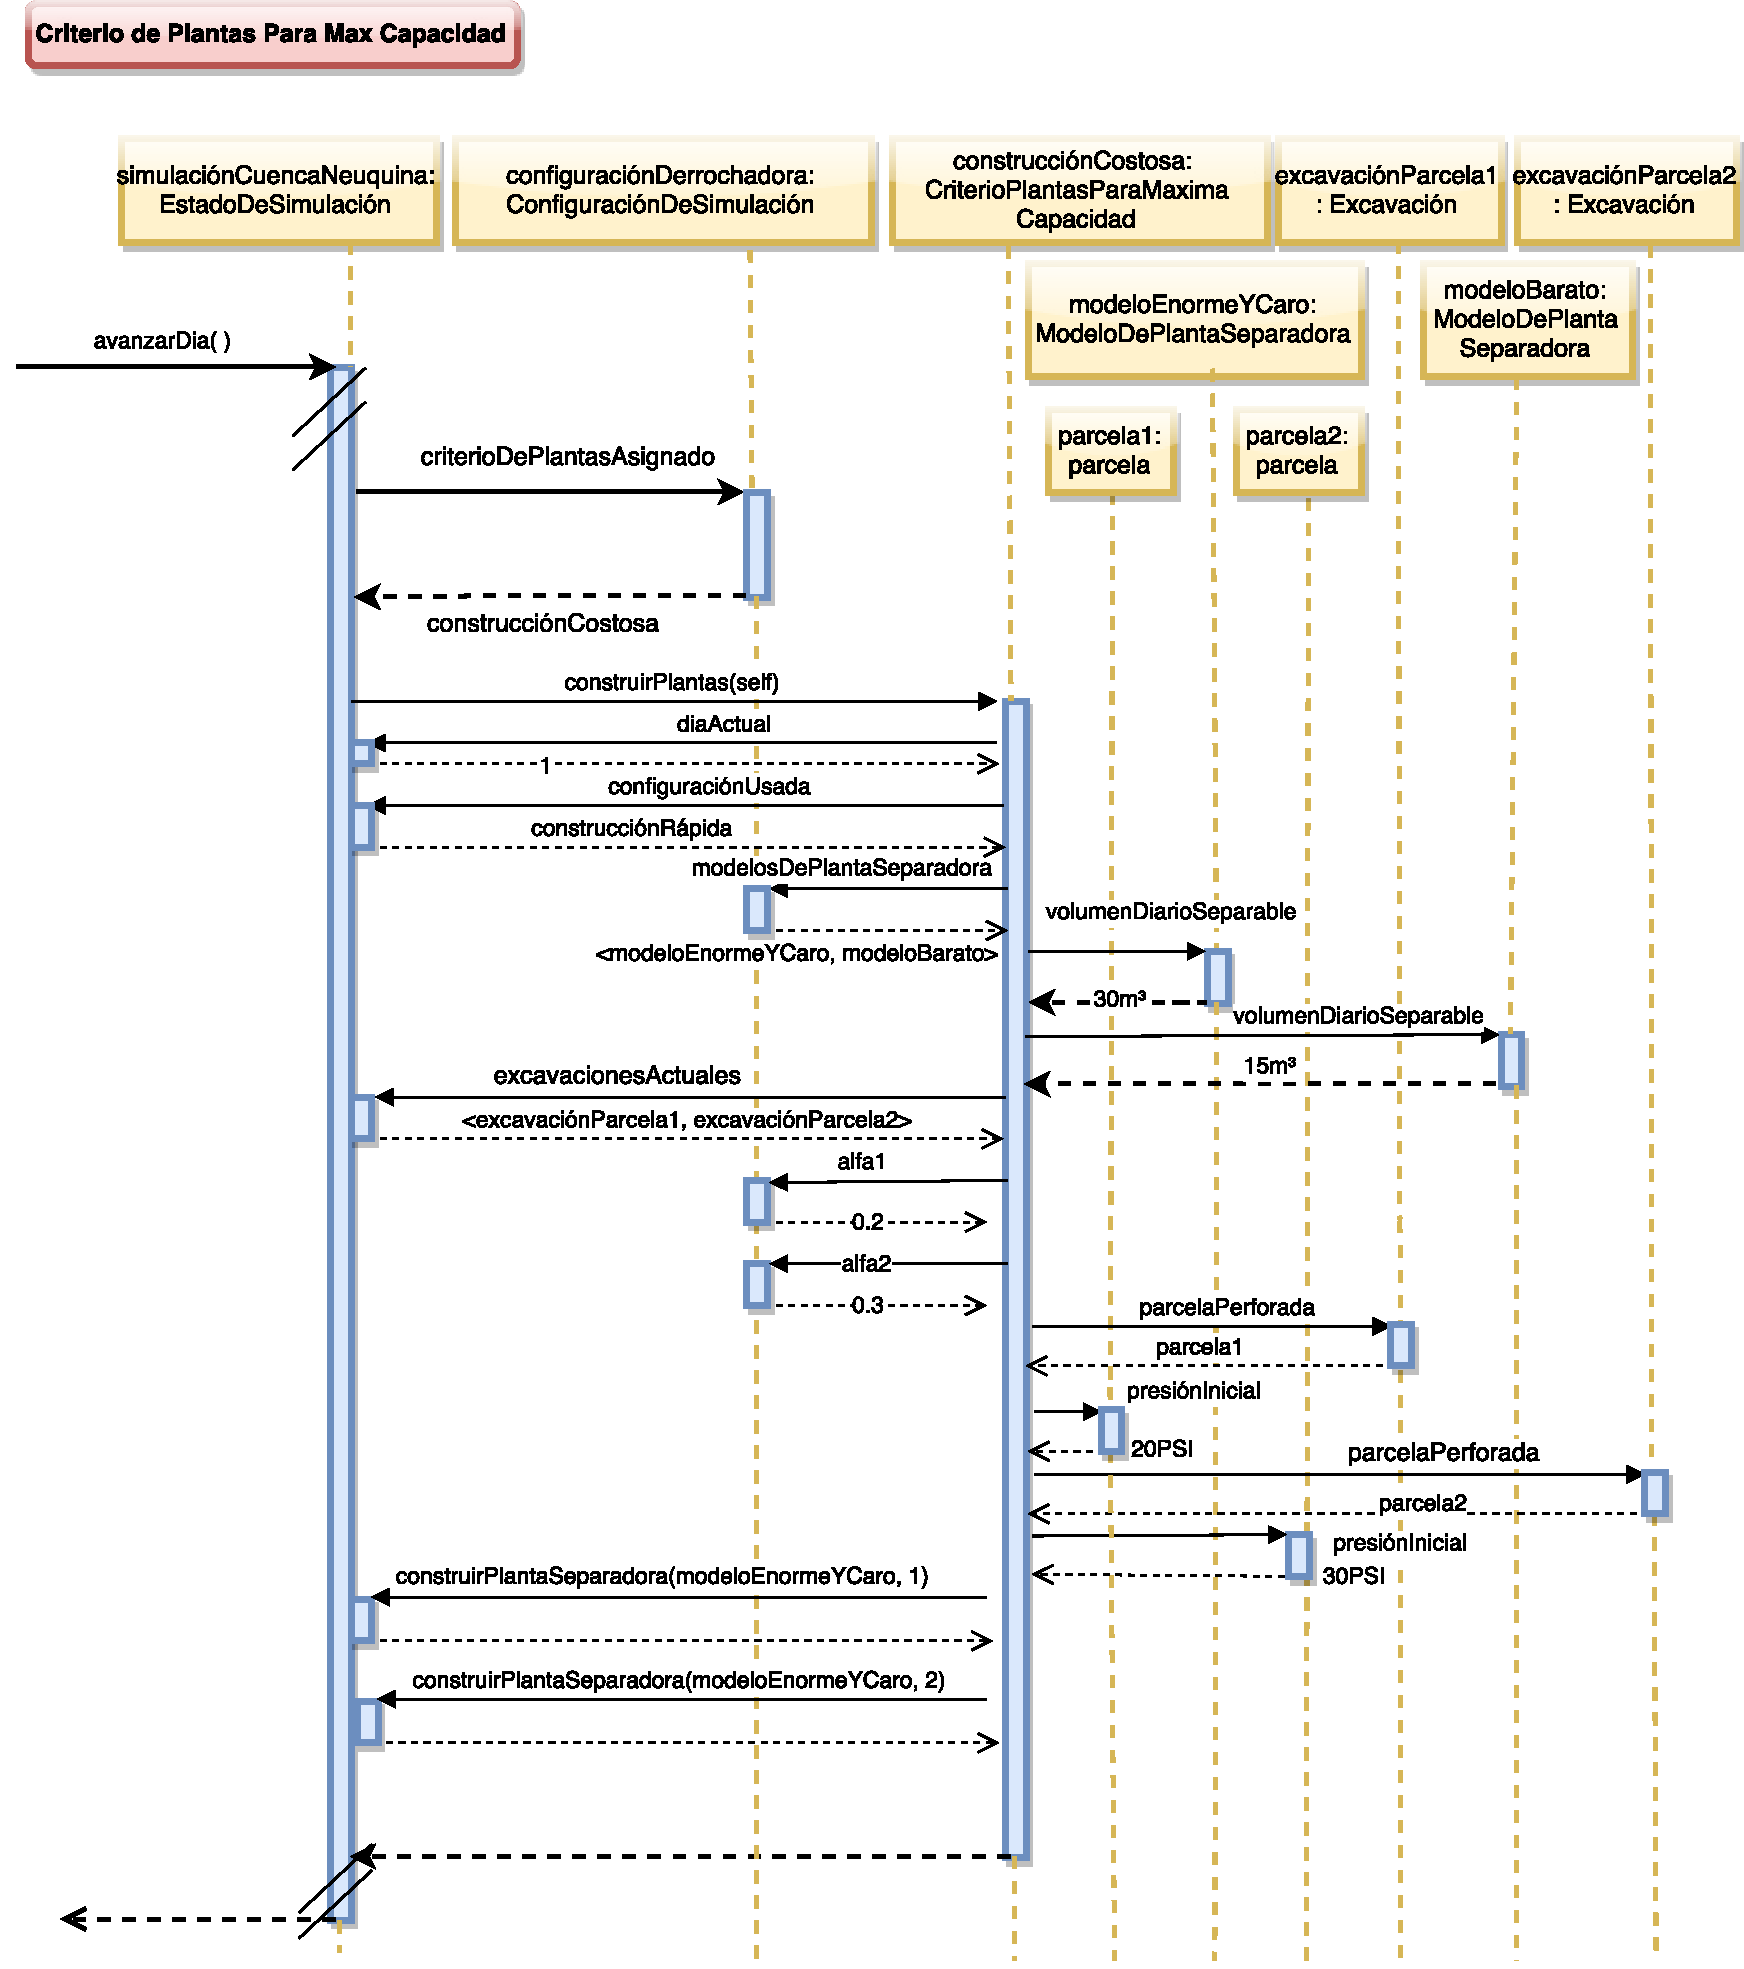
\includegraphics[width=1.15\textwidth, keepaspectratio]{plantas}
\end{figure}

En este diagrama el estado le delega al criterio constructor de plantas de la configuración la construcción de las mismas. Por tratarse de un criterio para máxima capacidad, el criterio calcula y construye la cantidad de plantas del modelo con mayor volumen diario separable necesarias para soportar el volumen extraído en todos los pozos en excavación el primer día de su funcionamiento. En este caso el criterio construye dos plantas del modelo más grande (también más costoso, como sería de esperar) tras haber consultado la presión inicial de las parcelas excavadas y los coeficientes de la configuración para calcular el volumen extraíble al primer día.
\\

El criterio de ahorro hace lo mismo pero solamente construye considerando la mitad de todo el producto extraíble el primer día de todos los pozos. Además se elige la planta con mayor ratio performance/costo en vez de la de mayor volumen diario separable.
\\

Las mismas colaboraciones se efectúan en los criterios de tanques (tanto para agua como para gas) salvo que se aplica la composición crítica al producto del primer día. De esta manera, se preparan tanques para la mayor cantidad de producto, pero considerando la composición más diluida posible (se asume que todo lo que no sea petróleo en la composición crítica es agua o gas según el tipo de tanque construido) lo que aporta una cota máxima al volumen de cada elemento almacenable por día. 
\\

%%%%%%%%%%%%%%%%%%%%%%%%%%%%%%%%%%%%%%%%%%%%%%%%%

\newpage
\textbf{Diagrama de criterio de contratación y asignación de RIGS}

\begin{figure}[H]
\centering
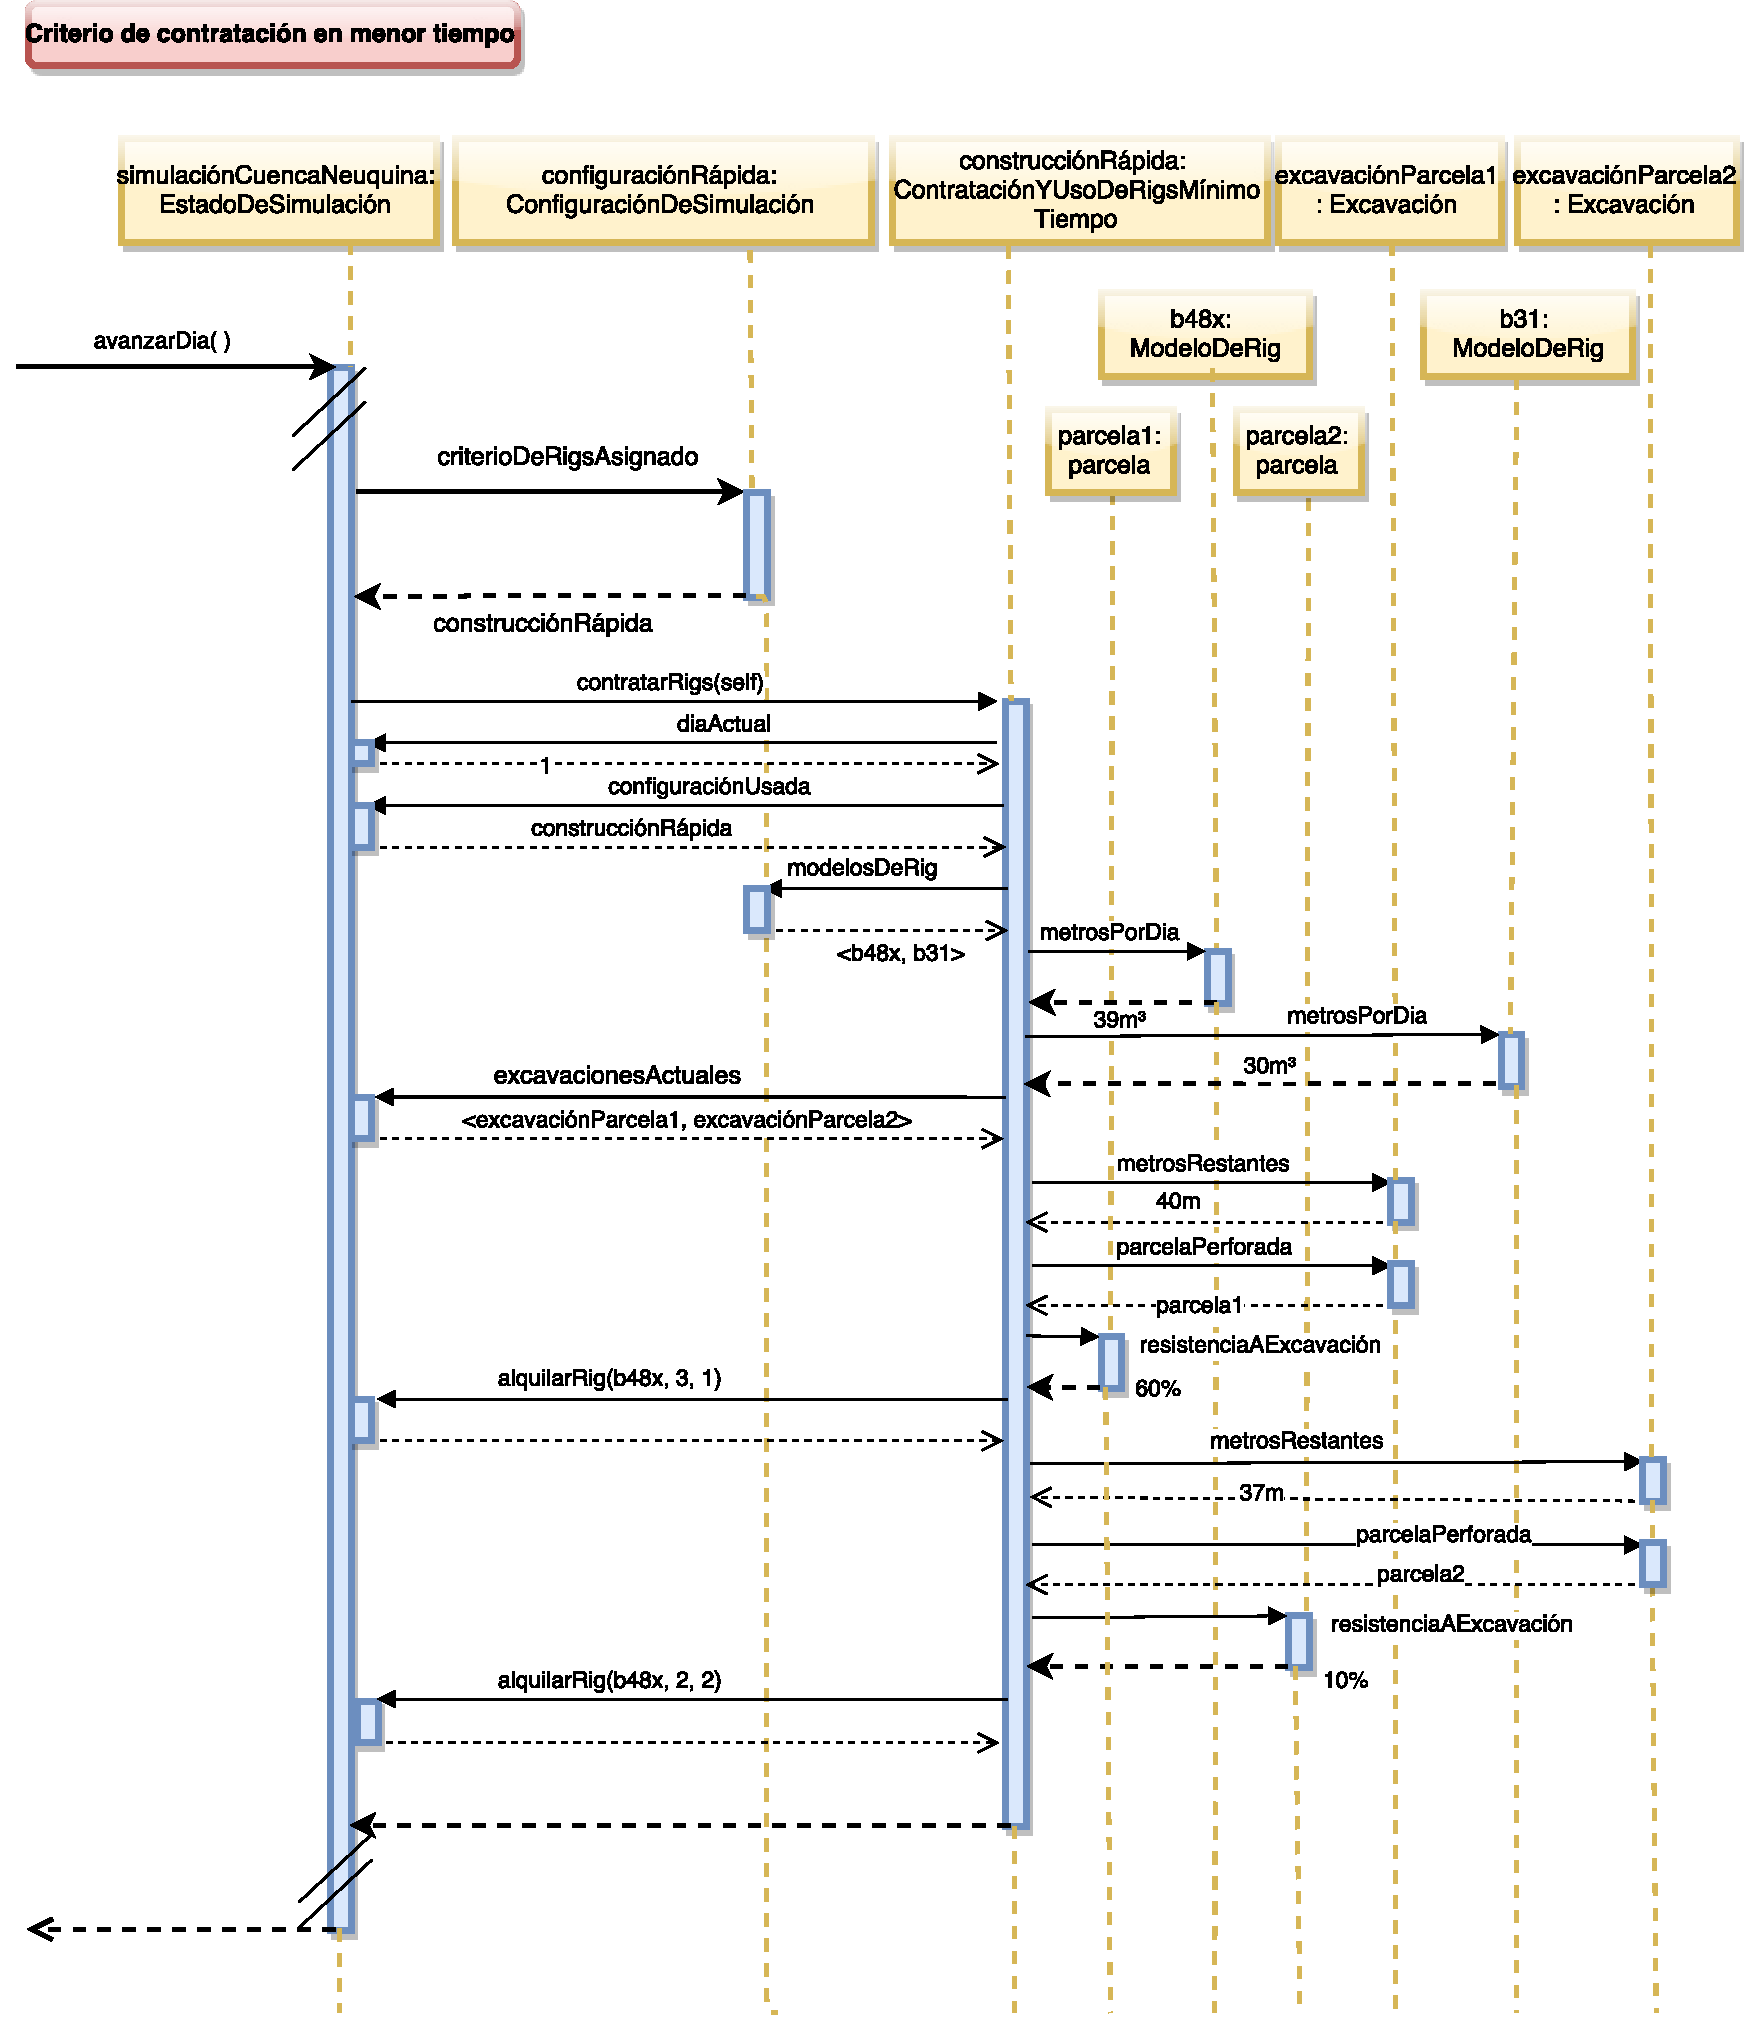
\includegraphics[width=1\textwidth, keepaspectratio]{rigs}
\end{figure}

Al igual que el criterio de construcción de plantas, el criterio de contratación se encarga de hacer todas las contrataciones necesarias el primer día. El resto de los días no contrata.
\\

Sabiendo el modelo de rig con más poder de excavación, el criterio de mínimo tiempo calcula cuántos días se necesitan para terminar de excavar todas las parcelas con este tipo de rig. De esta manera, las excavaciones terminan en el menor tiempo posible (aunque posiblemente alquilando los rigs más costosos).
\\

El mismo criterio luego responde al mensaje excavar simplemente asignando cualquiera de estos rigs con máximo poder de excavación a cada excavación existente (por la manera en que se contrata, siempre hay tantos rigs como excavaciones).
\\

En la versión de mínimo costo, se usa un único rig con menor costo final (es decir, ponderando consumo de combustible, costo de alquiler y días mínimos de alquiler) para realizar todas las excavaciones, aumentando tiempo pero también disminuyendo costos.

%%%%%%%%%%%%%%%%%%%%%%%%%%%%%%%%%%%%%%%%%%%%%%%%%

\newpage
\textbf{Diagrama de elección de parcelas}
\begin{figure}[H]
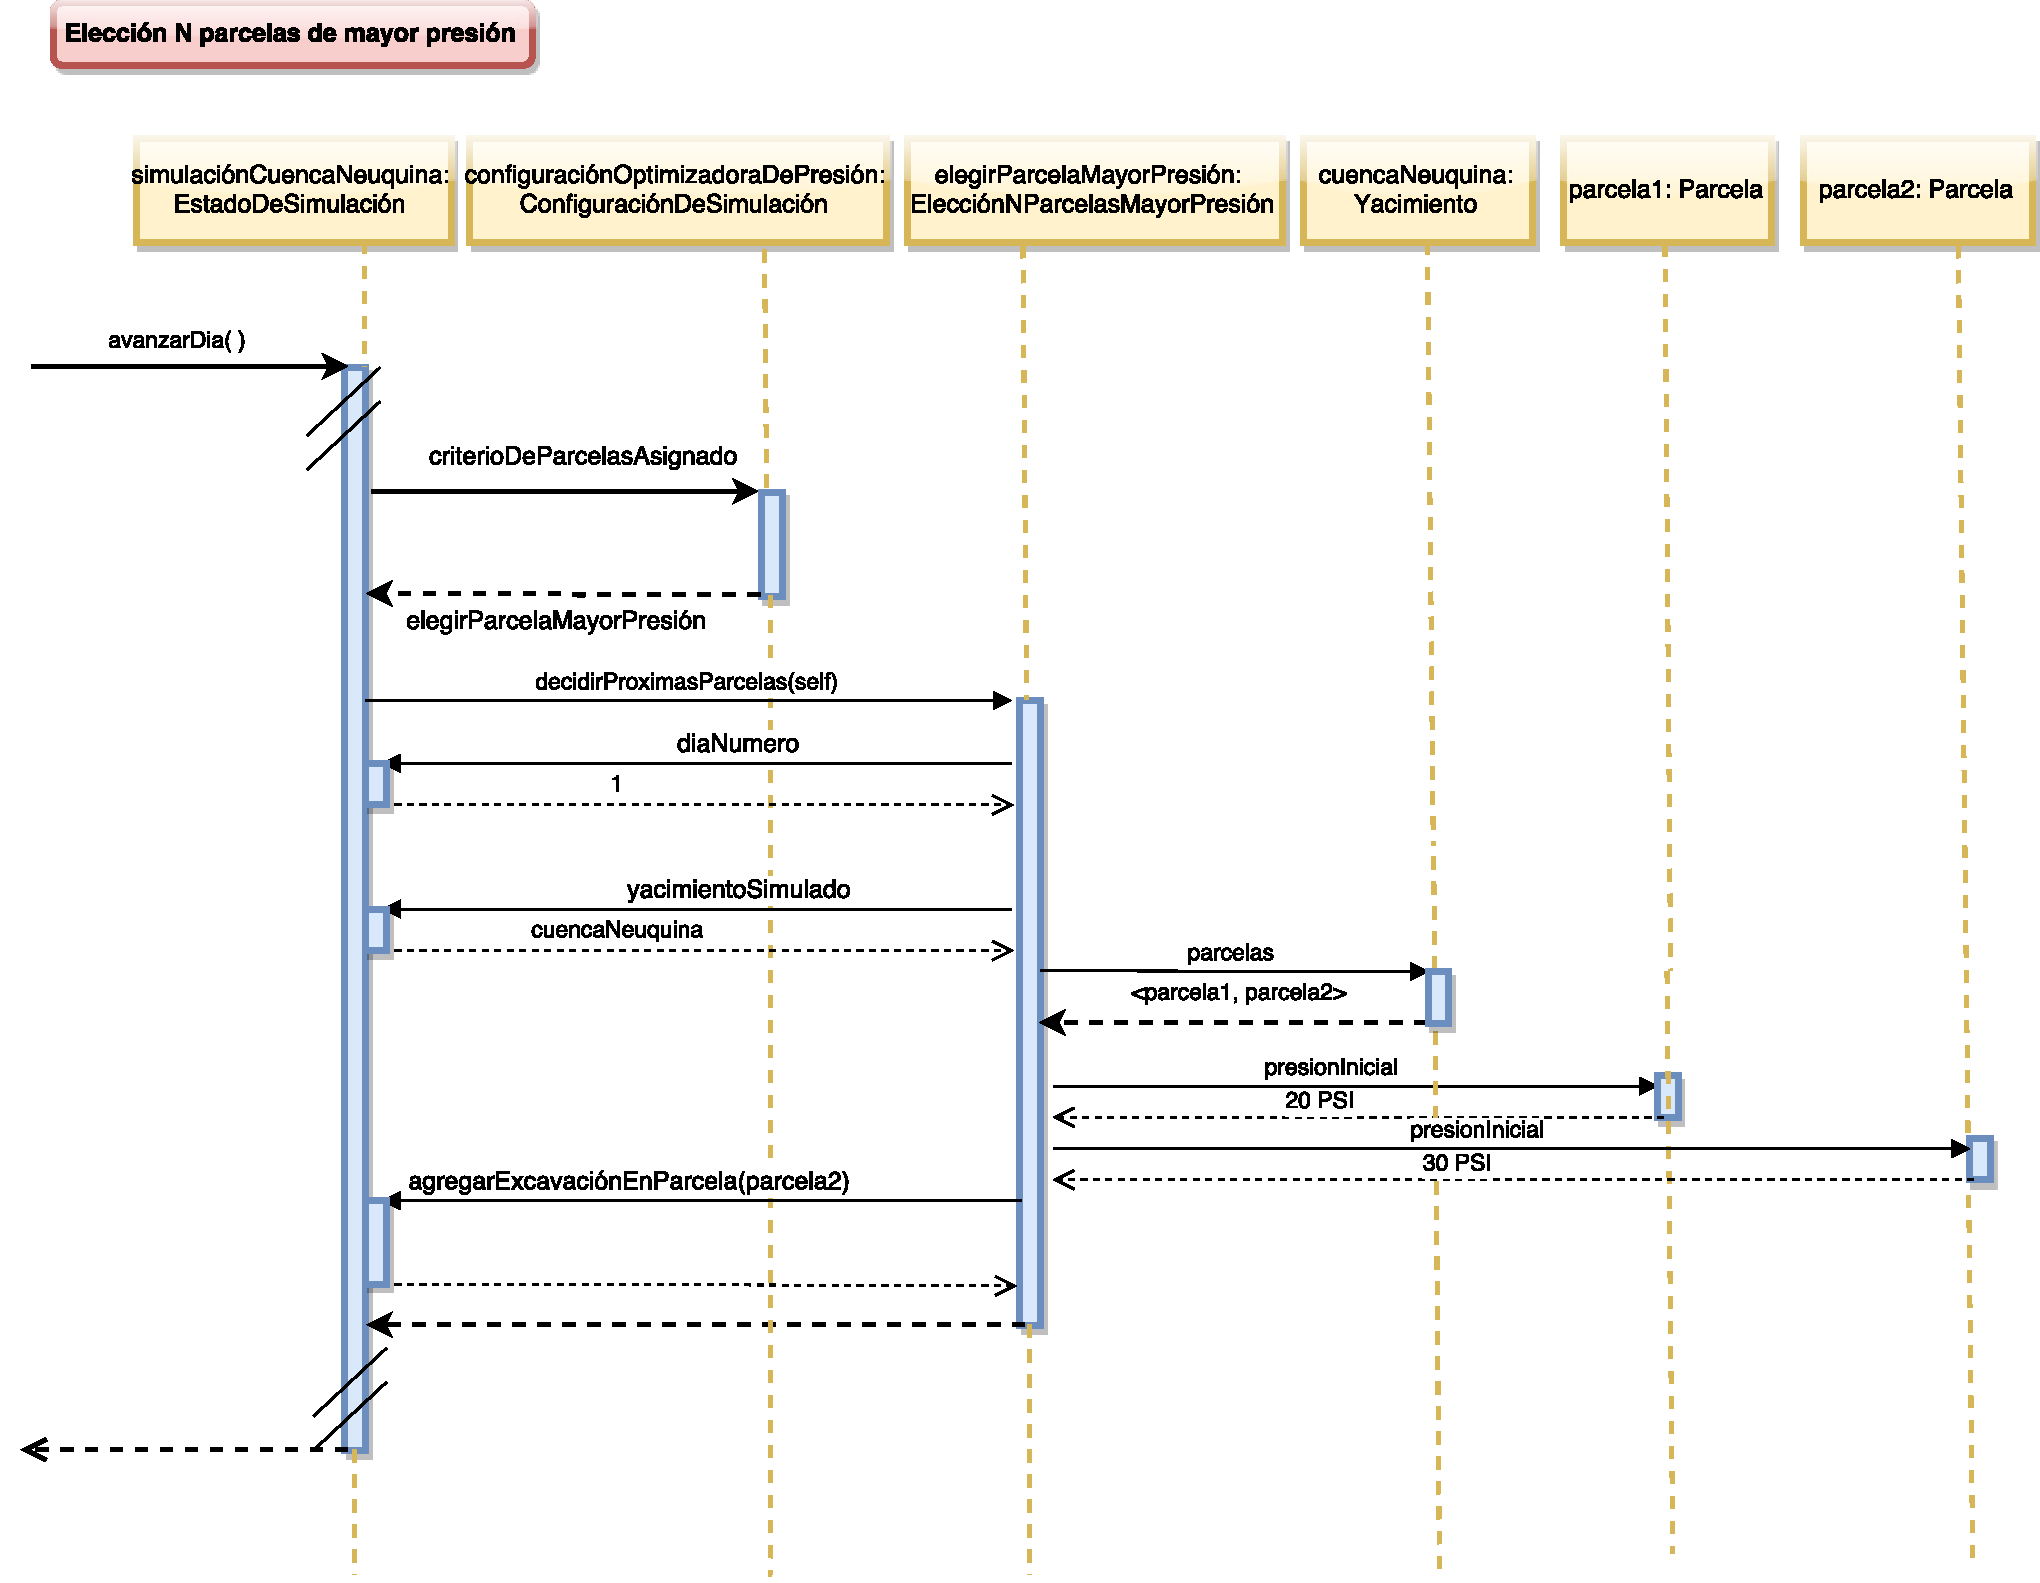
\includegraphics[width=1.15\textwidth, keepaspectratio]{parcelas}
\end{figure}

Cuando el estado de simulación llama al mensaje de decisión de las próximas parcelas a excavar el primer día, el criterio se encarga de consultar por el yacimiento simulado y, luego, por las parcelas que tiene. En el escenario del diagrama el criterio elige por mayor presión y la cantidad de parcelas elegibles prefijadas es 1, por lo tanto elige de las dos parcelas del yacimiento la parcela 2, que tiene mayor presión.
\\

En el caso del criterio que escoge N parcelas por profundidad, en lugar de preguntar por la presión inicial pregunta por la profundidad y escoge las N menores.
\\

Dado que el criterio elige el primer día la cantidad necesaria para el desarrollo de la explotación, el resto de los días no realiza nada en particular al recibir el mensaje.
\\

%%%%%%%%%%%%%%%%%%%%%%%%%%%%%%%%%%%%%%%%%%%%%%%%%

\newpage
\textbf{Diagrama de habilitación y extracción de pozos}
\begin{figure}[H]
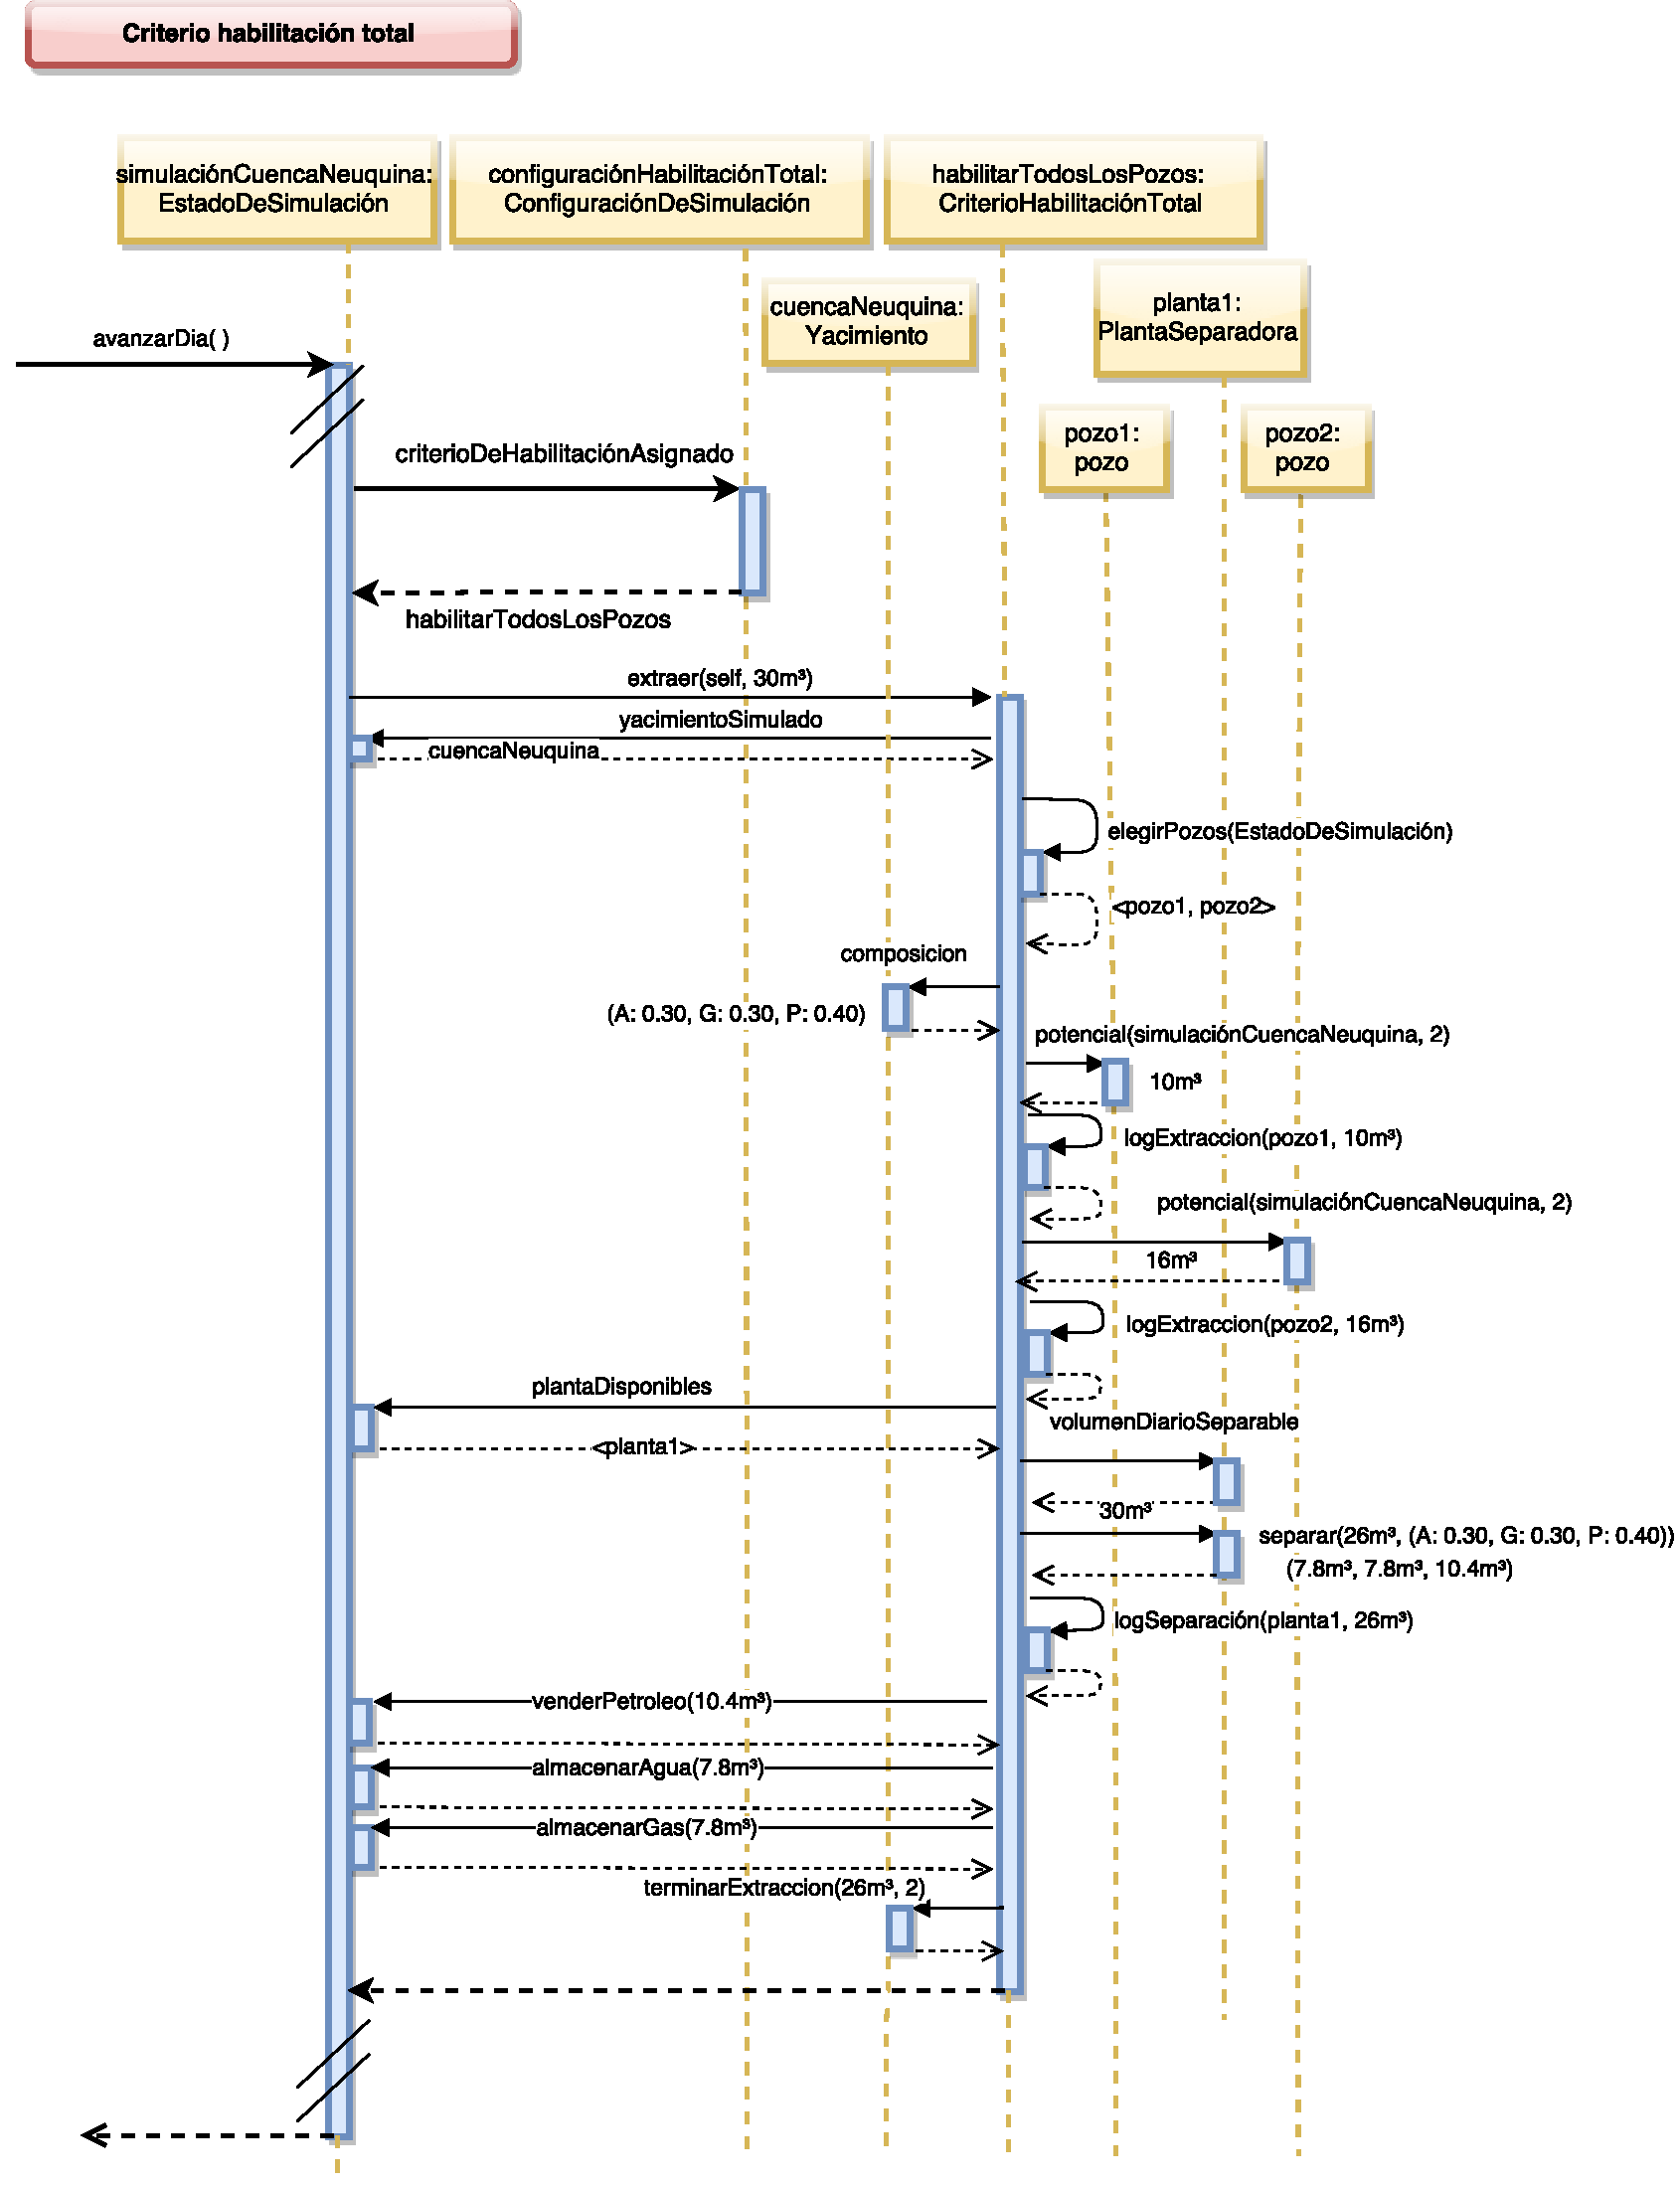
\includegraphics[width=0.9\textwidth, keepaspectratio]{extraccion}
\end{figure}

Cuando el estado envía el mensaje \emph{extraer} al criterio de habilitación de pozos este último consulta al primero por el yacimiento simulado para conocer su composición (lo conoce porque se envía como self junto con el tope de volumen extraible).
\\

El tope de volumen el estado lo calcula sabiendo tanto el volumen separable (conocimiento que consigue de sus plantas) y almacenable tanto de agua y gas (conocimiento que consigue de sus tanques y de la composición del yacimiento) de modo que todo lo extraído sea tanto separable como almacenable (ni el gas ni el agua se pueden tirar).
\\

También se autoenvía el mensaje \emph{elegirPozos} (el cual a diferencia de \emph{extraer} es implementado por cada criterio en particular) para saber cuáles son los pozos que tiene que iterar consultando por su potencial volumen. Por ser un criterio de habilitación total, elige los únicos dos pozos de la explotación. Si fuera la versión de N pozos de mayor presión, por ejemplo con N=1, hubiera elegido el pozo de los dos que mayor presión tuviera.
\\

Luego, conociendo las plantas del estado, se iteran para separar el total del producto extraído y finalmente indicándole al estado que venda el petróleo extraído y que almacene la cantidad de agua y gas extraída.
\\

Finalmente el criterio le indica al yacimiento que termine la extracción actualizando las presiones según la cantidad de pozos que se habilitó y el volumen que se extrajo.

%%%%%%%%%%%%%%%%%%%%%%%%%%%%%%%%%%%%%%%%%%%%%%%%%



\appendix

%\newpage
%\bibliography{bibliography}{}
%\bibliographystyle{plain}

\end{document}
